\chapter{Experimental Setup}
\label{chap_setup}
The data analyzed in this thesis is p-Pb collisions at $\sqrt{s_{NN}}=$ 5.02 TeV in Large Hadron Collider (LHC).
LHC is a high energy hadron collider for pp, p-Pb, and Pb-Pb collisions located at CERN. 
The data was collected by the ALICE detectors in 2013 winter. 

In this chapter, the experimental set up of this thesis is described. 
Most of the parts of the detector performance is referred to the ALICE Physics Report I, II and Performance of the ALICE Experiment at the CERN LHC~\cite{bib_aprv1,bib_aprv2,bib_aprrun1}. 


\section{The Large Hadron Collider (LHC)}
\label{sec_3_LHC}
The Large Hadron Collider (LHC) is the largest particle accelerator in the world. 
The accelerator occupies the 27 km underground circular tunnel across the border between Switzerland and France which was formerly used for the Large Electron-Positron Collider (LEP). 
LHC can store and accelerate the various hadrons with 16 radio-frequency (RF) accelerating cavities and over 1600 superconducting magnets. 
The design energy of collided proton and lead is 7 TeV and 2.75 TeV/nucleon, respectively.

LHC hosts the 4 main experiments, ATLAS, CMS, LHCb, and ALICE which focus on different high energy particle and nuclear physics. 
ATLAS (A Toroidal LHC Apparatus), CMS (Compact Muon Solenoid), and ALICE (A Large Ion Collider Experiment) collected the data of the heavy ion collisions during Run1 (2009 - 2013) and contribute various progress related to the QGP physics. 
LHCb also took p-Pb collision data in 2013 and have a plan to take the heavy ion collision data from Run2 (2016-).

Figure~\ref{fig_3_lhc} shows the schematics view of the CERN accelerator complex~\cite{bib_cernaccel}. 
Protons are accelerated by a linear accelerator LINAC2. Before injected into the Proton Synchrotron (PS), the booster accelerate them to 1.4 GeV. 
They are sent PS and Super Proton Synchrotron (SPS) sequentially and accelerated to 450 GeV. 
And then they are transferred to two rings of LHC.
They go around the two rings in the opposite direction. 
Lead ions are also accelerated in similar process but there are some differences.
Lead ions are generated by heating a highly purified lead sample up to around 550.
At this stage, $Pb^{27+}$ is dominant. 
They are accelerated via LINAC3 and pass through the carbon foil which strips them to $Pb^{+54}$. 
They are also accelerated via Low Energy Ion Ring (LEIR) before injected into PS up to 72 MeV per nucleon.
PS accelerate them 5.9 GeV per nucleon and they are transferred into the foil again and fully stripped. 
The fully stripped ions are accelerated at SPS up to 177 GeV and sent to LHC rings. 
The injected protons and leads are further accelerated by LHC and finally two opposite beams of protons or heavy ions are delivered and collide at four interaction points of main experiments.
During Run1, pp at $\sqrt{s}=$ 900 GeV, 2.76 TeV, 7 TeV, and 8 TeV, p-Pb $\sqrt{s_{NN}}=$ 5.02 TeV and Pb-Pb $\sqrt{s_{NN}}=$ 2.76 GeV were provided by LHC. 
\begin{figure}[!h]
  \centering
  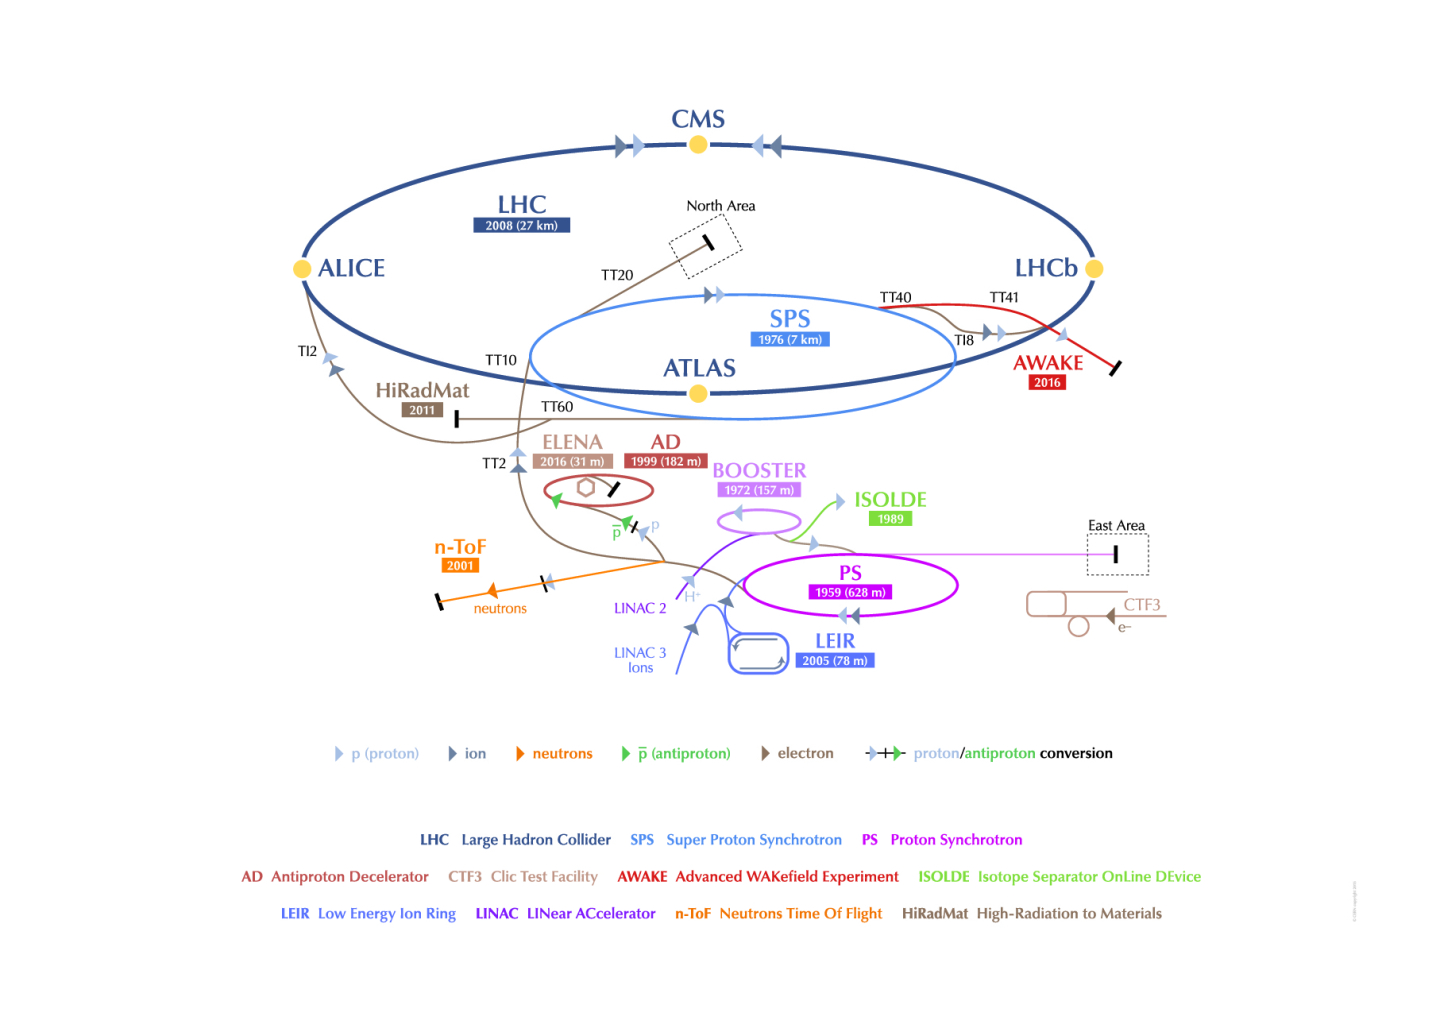
\includegraphics[width=12cm]{chap3/figure/LHC/CERNAcceleratorComplex.jpg}
  \caption{Schematics of CERN Accelerator Complex~\cite{bib_cernaccel}.}
  \label{fig_3_lhc}
\end{figure}


\section{Overview of the ALICE Detectors}
\label{sec_3_ALICE}
A Large Ion Collider Experiment (ALICE) is one of the major experiments in LHC dedicated heavy ion collisions. 
The all data analyzed in this thesis is collected with the ALICE detectors. 

Figure~\ref{fig_3_alicefigure} shows the schematics of ALICE detectors. 
In order to cope with high particle multiplicity in heavy ion collision events (up to $dN/d\eta \sim$ 8000) and cover a wide momentum active range with excellent particle identification, various detectors with high granularity and good PID performance in specific momentum ranges are installed in the central barrel and combined analysis for these detectors is performed. 
%The number of readout channels is enormous and the data size of one heavy collision reaches. 
%The data bandwidth is assumed. 

The determination of event characteristics is crucial to study heavy ion physics as discussed in Chapter~2.
V0, FMD, and ZDC are mainly aimed to determine the event centrality.  
The acceptance and main technology of each detector is summarized in Table~\ref{table_3_alicedet}. 
The detail of the detectors related to this thesis is described from the next section. 

\begin{figure}[!h]
  \centering
  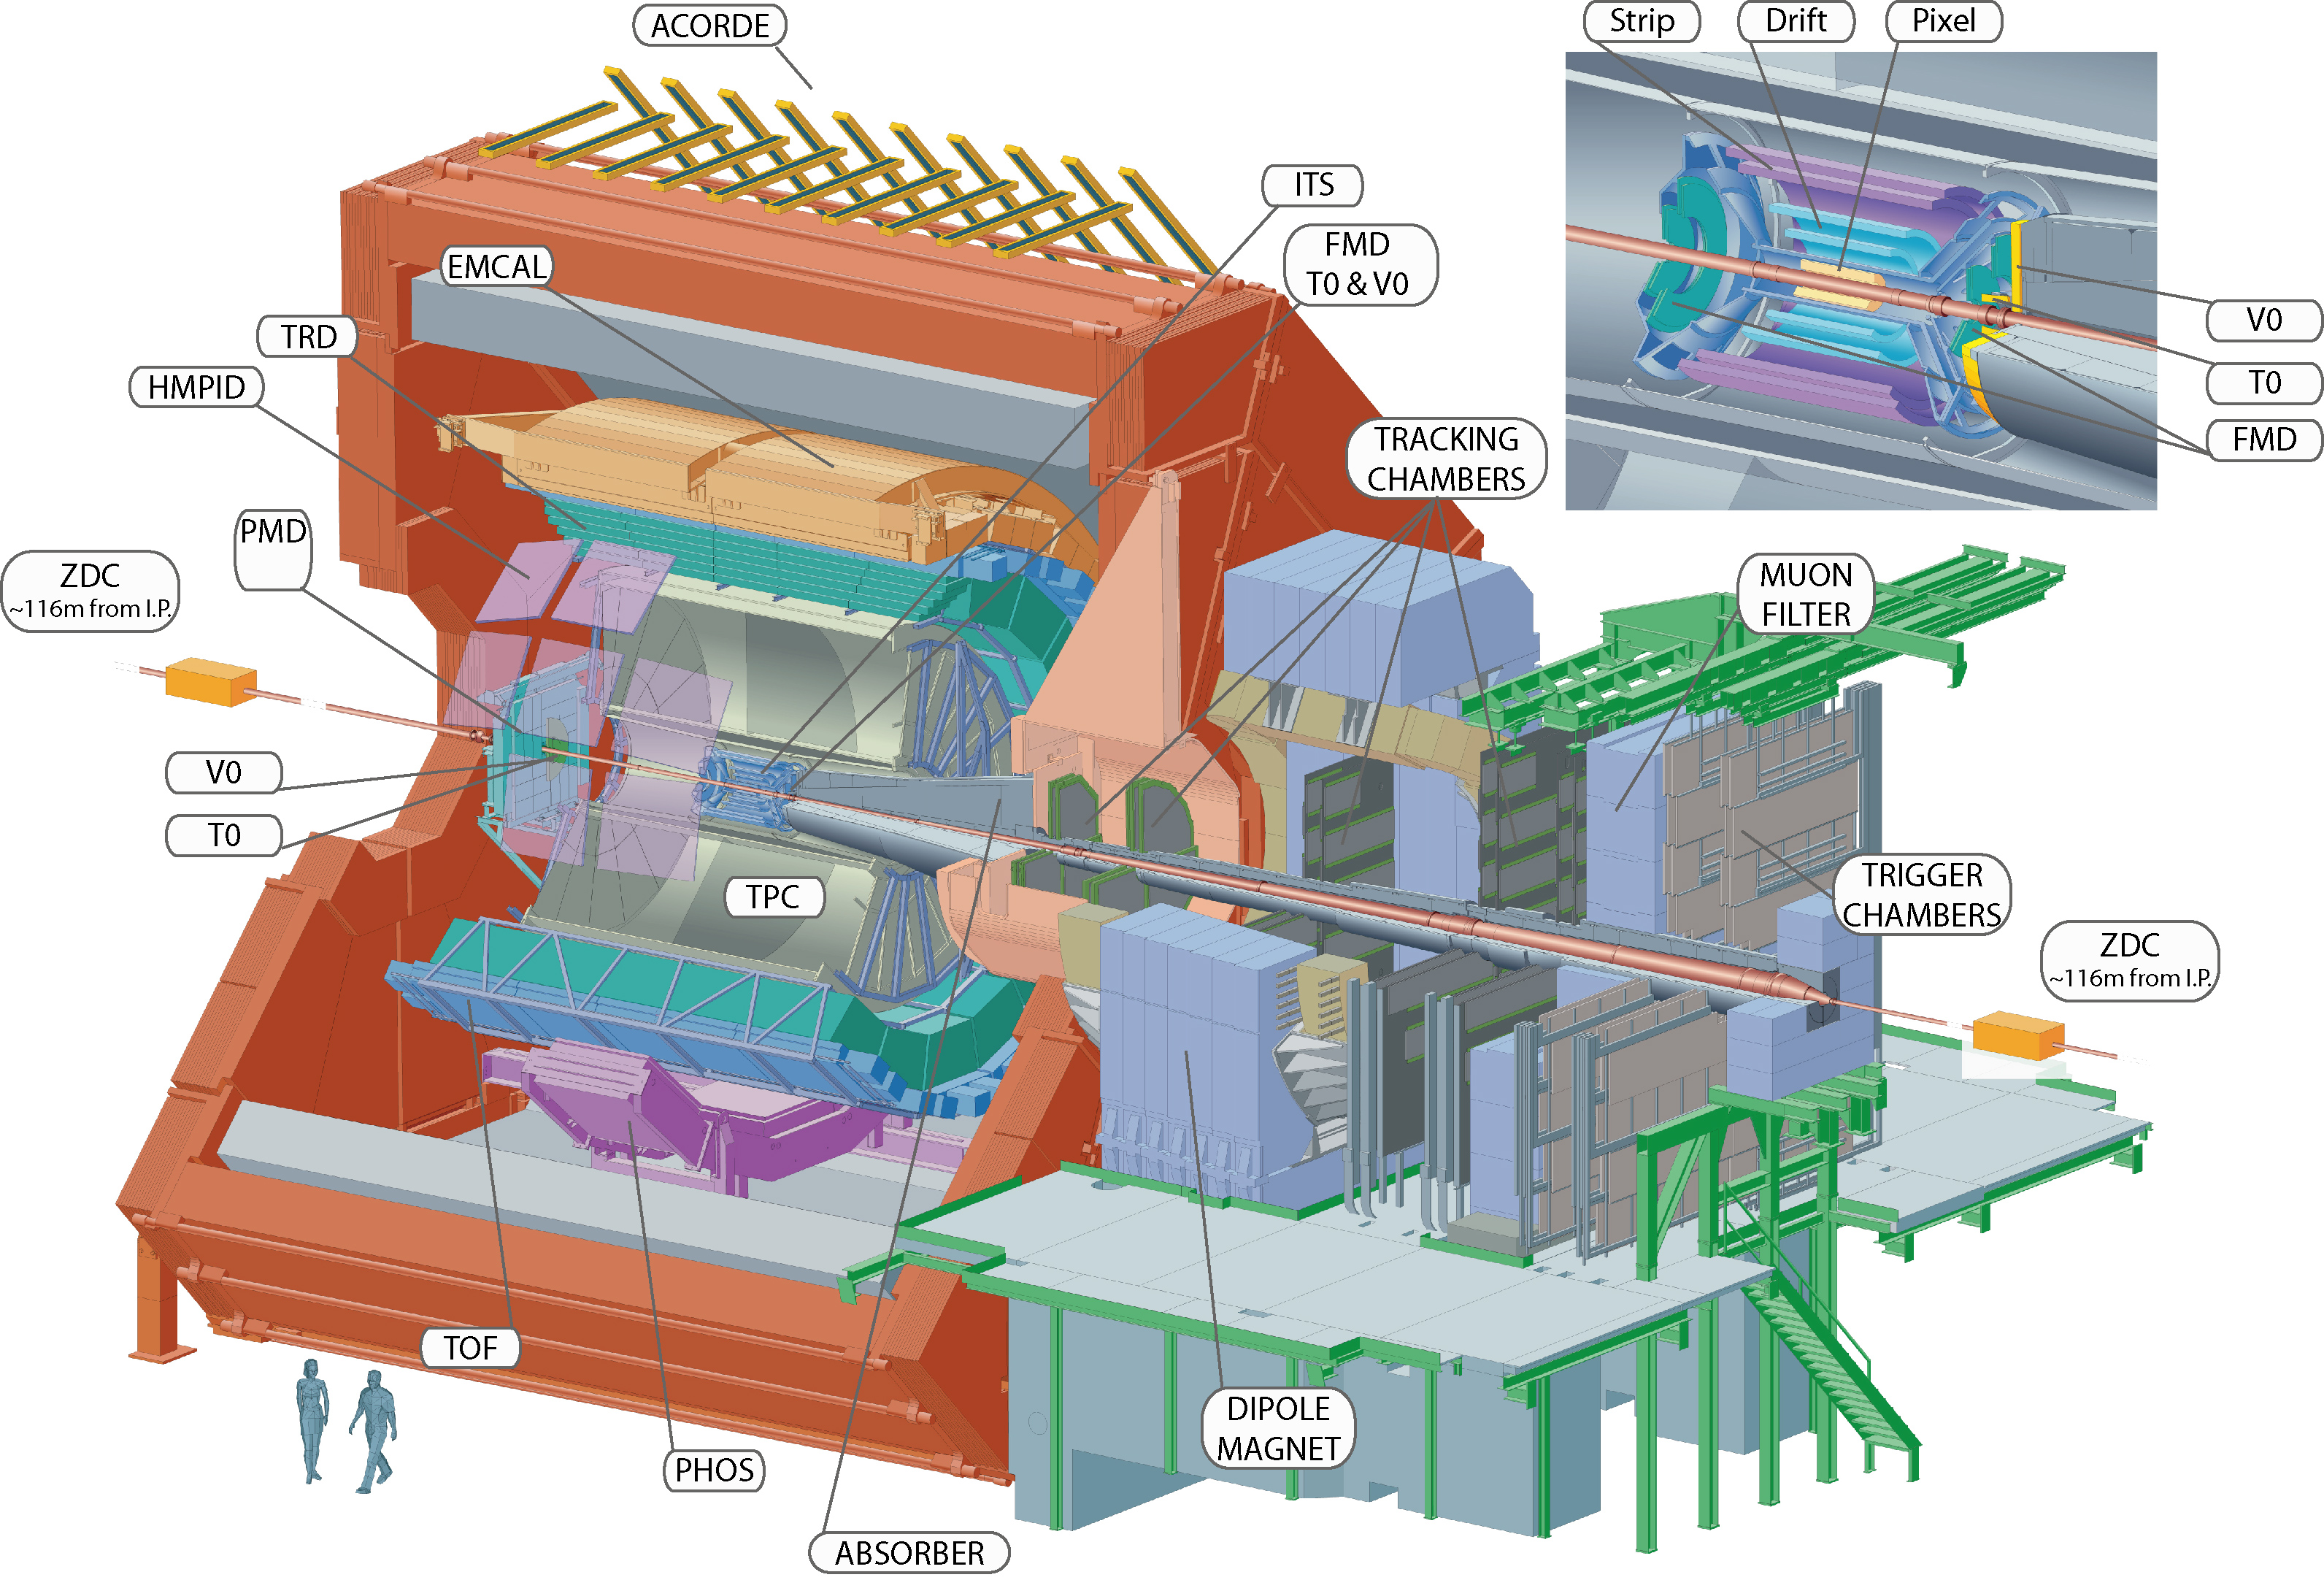
\includegraphics[width=15cm]{chap3/figure/ALICE/ALICE_Schematics.jpg}
  \caption{Schematics of ALICE detectors~\cite{bib_aprrun1}.}
  \label{fig_3_alicefigure}
\end{figure}

\begin{table}[!htb]
  \centering
  \small
    \begin{tabular}{|r|c|c|c|c|} \hline
    Detector & $\eta$ coverage  & $\phi$ coverage & Technology & Main Purpose \\ \hline
    ITS SPD & $|\eta| < $1.4 & full & Silicon & tracking, vertexing \\
    SDD & $|\eta| < $ 0.9  & full & Silicon & tracking, low pt PID \\
    SSD & $|\eta| < $ 1.0  & full & Silicon & tracking, low pt PID \\
    TPC & $|\eta| < $ 0.9  & full & Ne/Ar drift+MWPC & tracking, PID \\
    TRD & $|\eta| < $ 0.9  & full & TR+Xe drift+MWPC & tracking, electronPID \\
    TOF & $|\eta| < $ 0.9  & full & MRPC & PID \\
    EMCAL & $|\eta| < $ 0.7 & 80  $<\phi<$ 187  & Pb+scintillator & photon, electron ID, jet \\
    V0 V0A& 2.8 $< \eta < $ 5.1 & full & scintillator & L0, Multiplicity \\
    V0 V0C& -3.1 $< \eta < $ -1.7 & full & scintillator & L0, Multiplicity \\
    T0 T0A& 4.6 $< \eta < $ 4.9 & full & quartz & Timing, Vertexing \\ 
    T0 T0C& -3.3 $< \eta < $ -3.0 & full & quartz & Timing, Vertexing \\ 
    Muon Chamber & -4.0$<\eta < $-2.5 & full &MWPC &Muon tracking \\	  
    Muon Trigger & -4.0$<\eta < $-2.5 & full &RPC &Muon trigger \\ \hline  	     
      \end{tabular}
 \caption{ Summary of acceptance and main technology for subdetectors in ALICE~\cite{bib_aprrun1}.}
  \label{table_3_alicedet}
\end{table}

In this thesis, the global coordinate system in ALICE is defined as shown Fig.~\ref{fig_3_alicecood}. 
It is a right-handed coordinate system with Z-axis. 
The Z-axis is parallel to the mean beam direction. 
The positive Z-axis is the opposite direction of the Muon arm, called 'A-side'. 
On the other hand, 'C-side' is defined as the opposite side of A-side. 
\begin{figure}[!h]
  \centering
  \includegraphics[width=10cm]{chap3/figure/ALICE/ALICE_Coordinate.png}
  \caption{Global coordinate of ALICE detectors~\cite{bib_aprv2}.}
  \label{fig_3_alicecood}
\end{figure}


\section{ALICE Global Detectors}
\label{sec_3_ALICEglobal}
\subsection{V0 Detector}
The V0 detector is a scintillation detector used for the minimum bias trigger decision and the determination of event characteristics mainly. 
V0 is formed of V0A and V0C on either side of the interaction point. 
V0A is located 340 cm away from the interaction point and covers 2.8 $< \eta < $ 5.1. 
V0C is also installed 90 cm from the interaction point and covers -3.1 $< \eta < $ -1.7.
They have 4 and 8 segments in the r and $\phi$ direction, respectively as shown in Fig.~\ref{fig_3_v0det}. 

\begin{figure}[!h]
  \centering
  
\includegraphics[width=6cm]{chap3/figure/V0/CrossSection_V0.png}
  \caption{Segmentation of V0 detector~\cite{bib_aprv1}.}
  \label{fig_3_v0det}
\end{figure}

The event centrality and the event plane is estimated via measurements of the charge particle multiplicity in each segment of V0. 
Figure~\ref{fig_3_v0multi} shows the sum of V0A amplitude distribution in p-Pb collisions which is proportional to the charged particle multiplicity\cite{bib_v0multi}.
The red-line in Fig.~\ref{fig_3_v0multi} shows the result of NDB-Glauber fit~\cite{bib_ndbglauber1,bib_ndbglauber2,bib_ndbglauber3,bib_ndbglauber4}. 
The event centrality is determined by the percentile of this distribution. 
\begin{figure}[!h]
  \centering
  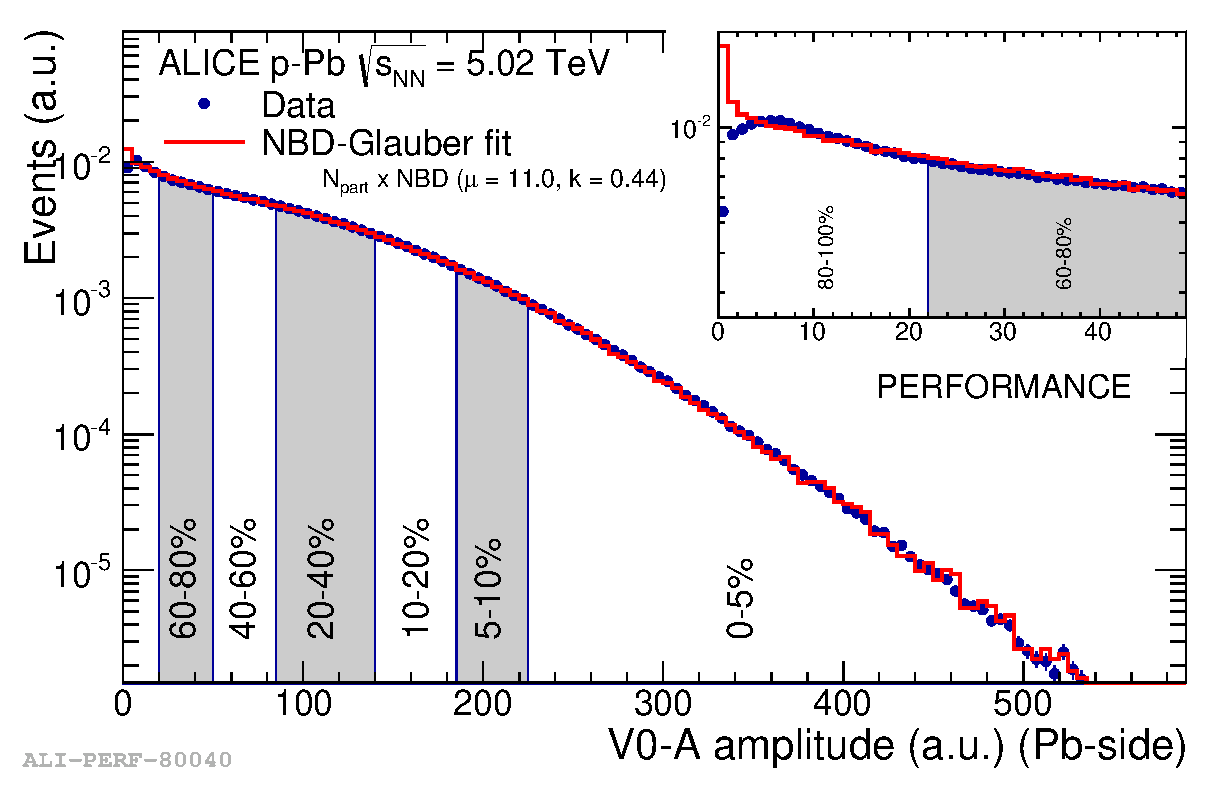
\includegraphics[width=10cm]{chap3/figure/V0/V0AMulti_pPb.eps}
  \caption{V0A multiplicity distribution in p-Pb collision at $\sqrt{s_{NN}}=$5.02 TeV (Pb-going side)~\cite{bib_v0multi}.}
  \label{fig_3_v0multi}
\end{figure}

The timing resolution of V0 is about 1 ns which enable to reject background events caused by beam-gas and beam-halo events. 


\subsection{T0 Detector}
The T0 detector is the arrays of Cherenkov counters to measure the collision time with high precision. 
The collision time is used as the reference time for TOF detector. 
The time resolution of T0 achieves 25 ps. 
T0 is also used of the determination of vertex position with a precision of about 1.5 cm. 
If the collision vertex reconstructed by T0 signal is inside the expected window, L0 trigger is issued.  
The signal from T0 also contribute to the pretrigger signal for TRD. 

\section{Detectors in ALICE Central Barrel}
\label{sec_3_ALICEcentral}
The main tracking detectors in the central barrel are ITS, TPC, and TRD. 
The strength of the solenoid magnet in the central barrel which was inherited from the former LEP experiment L3 is configurable 0.2-0.5 T in the direction of z-axis and the $p_{T}$ cut of charged particles is $p_{T}>$ 0.1 GeV/c. 
\subsection{Inner Tracking System (ITS)}
The Inner Tracking System (ITS) is the closest detector to the collision point. 
Figure~\ref{fig_3_itslayout} shows the layout of ITS. 
ITS consist of 6 layers of silicon detectors, two each of Silicon Pixel Detector (SPD), Silicon Drift Detector (SDD), Silicon Strip Detector (SSD). 
SPD is based on hybrid silicon pixels which consist of silicon detector diodes with thickness of 200 $\mu$m. 
SDD consists of a 300 $\mu$m  thick layer of homogeneous high-resistivity silicon. 
SSD is formed of double-sided silicon micro-strip sensors. 
The strip pitch is 95 $\mu$m  and the relative p-n side stereo angle is 35 mrad. 
ITS cover the full azimuthal acceptance and the pseudo-rapidity coverage of SPD and SDD is $|\eta|<$ 2.0 and $|\eta|<$ 0.9, respectively.  
The typical features of each layer detector is summarized in Table.~\ref{table_3_itsdet}. 
\begin{figure}[!h]
  \centering
  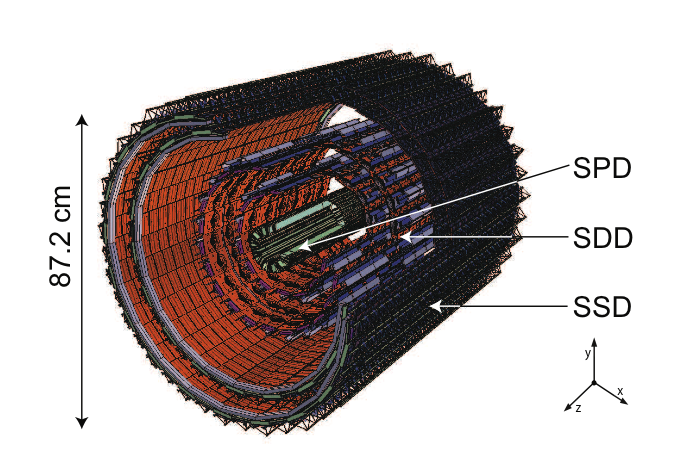
\includegraphics[width=10cm]{chap3/figure/ITS/Schematics_ITS.png}
  \caption{Schematics of ITS layout~\cite{bib_itstdr}.}
  \label{fig_3_itslayout}
\end{figure}

\begin{table}[!htb]
  \centering
  \begin{tabular}{|c|c|c|c|c|c|} \hline
    Layer & Detector Type  & Radius (cm) & Length (cm) & $\Delta$r$\phi$ ($\mu$m) & $\Delta$Z ($\mu$m) \\ \hline
    1     & SPD            & 3.9         & 28.2 & 12 & 100 \\ \hline 
    2     & SPD            & 7.6         & 28.2 & 12 & 100 \\ \hline
    3     & SDD            & 15.0        & 44.4 & 35 & 25 \\ \hline
    4     & SDD            & 23.9        & 59.6 & 35 & 25 \\ \hline
    5     & SSD            & 38.0        & 86.2 & 20 & 830 \\ \hline
    6     & SSD            & 43.0        & 97.8 & 20 & 830 \\ \hline
  \end{tabular}
  \caption{ Detector type and general features of each layer of ITS~\cite{bib_itstdr}.}
  \label{table_3_itsdet}
\end{table}

Figure~\ref{fig_3_firstpp} shows an example of ITS hits and track reconstruction in pp at $\sqrt{s_{NN}}=$ 900 GeV~\cite{bib_firstpp}. 
The main purpose of ITS is to determine the position of the primary vertex and secondary decay vertex. 
It is also useful for the precise determination of the impact parameters which enables to separate charm and bottom decay contributions by the difference of decay length. 
The offline tracking is done with combined information of ITS and TPC. 
ITS provide the reference to improve the momentum resolution of TPC. 

\begin{figure}[!h]
  \centering
  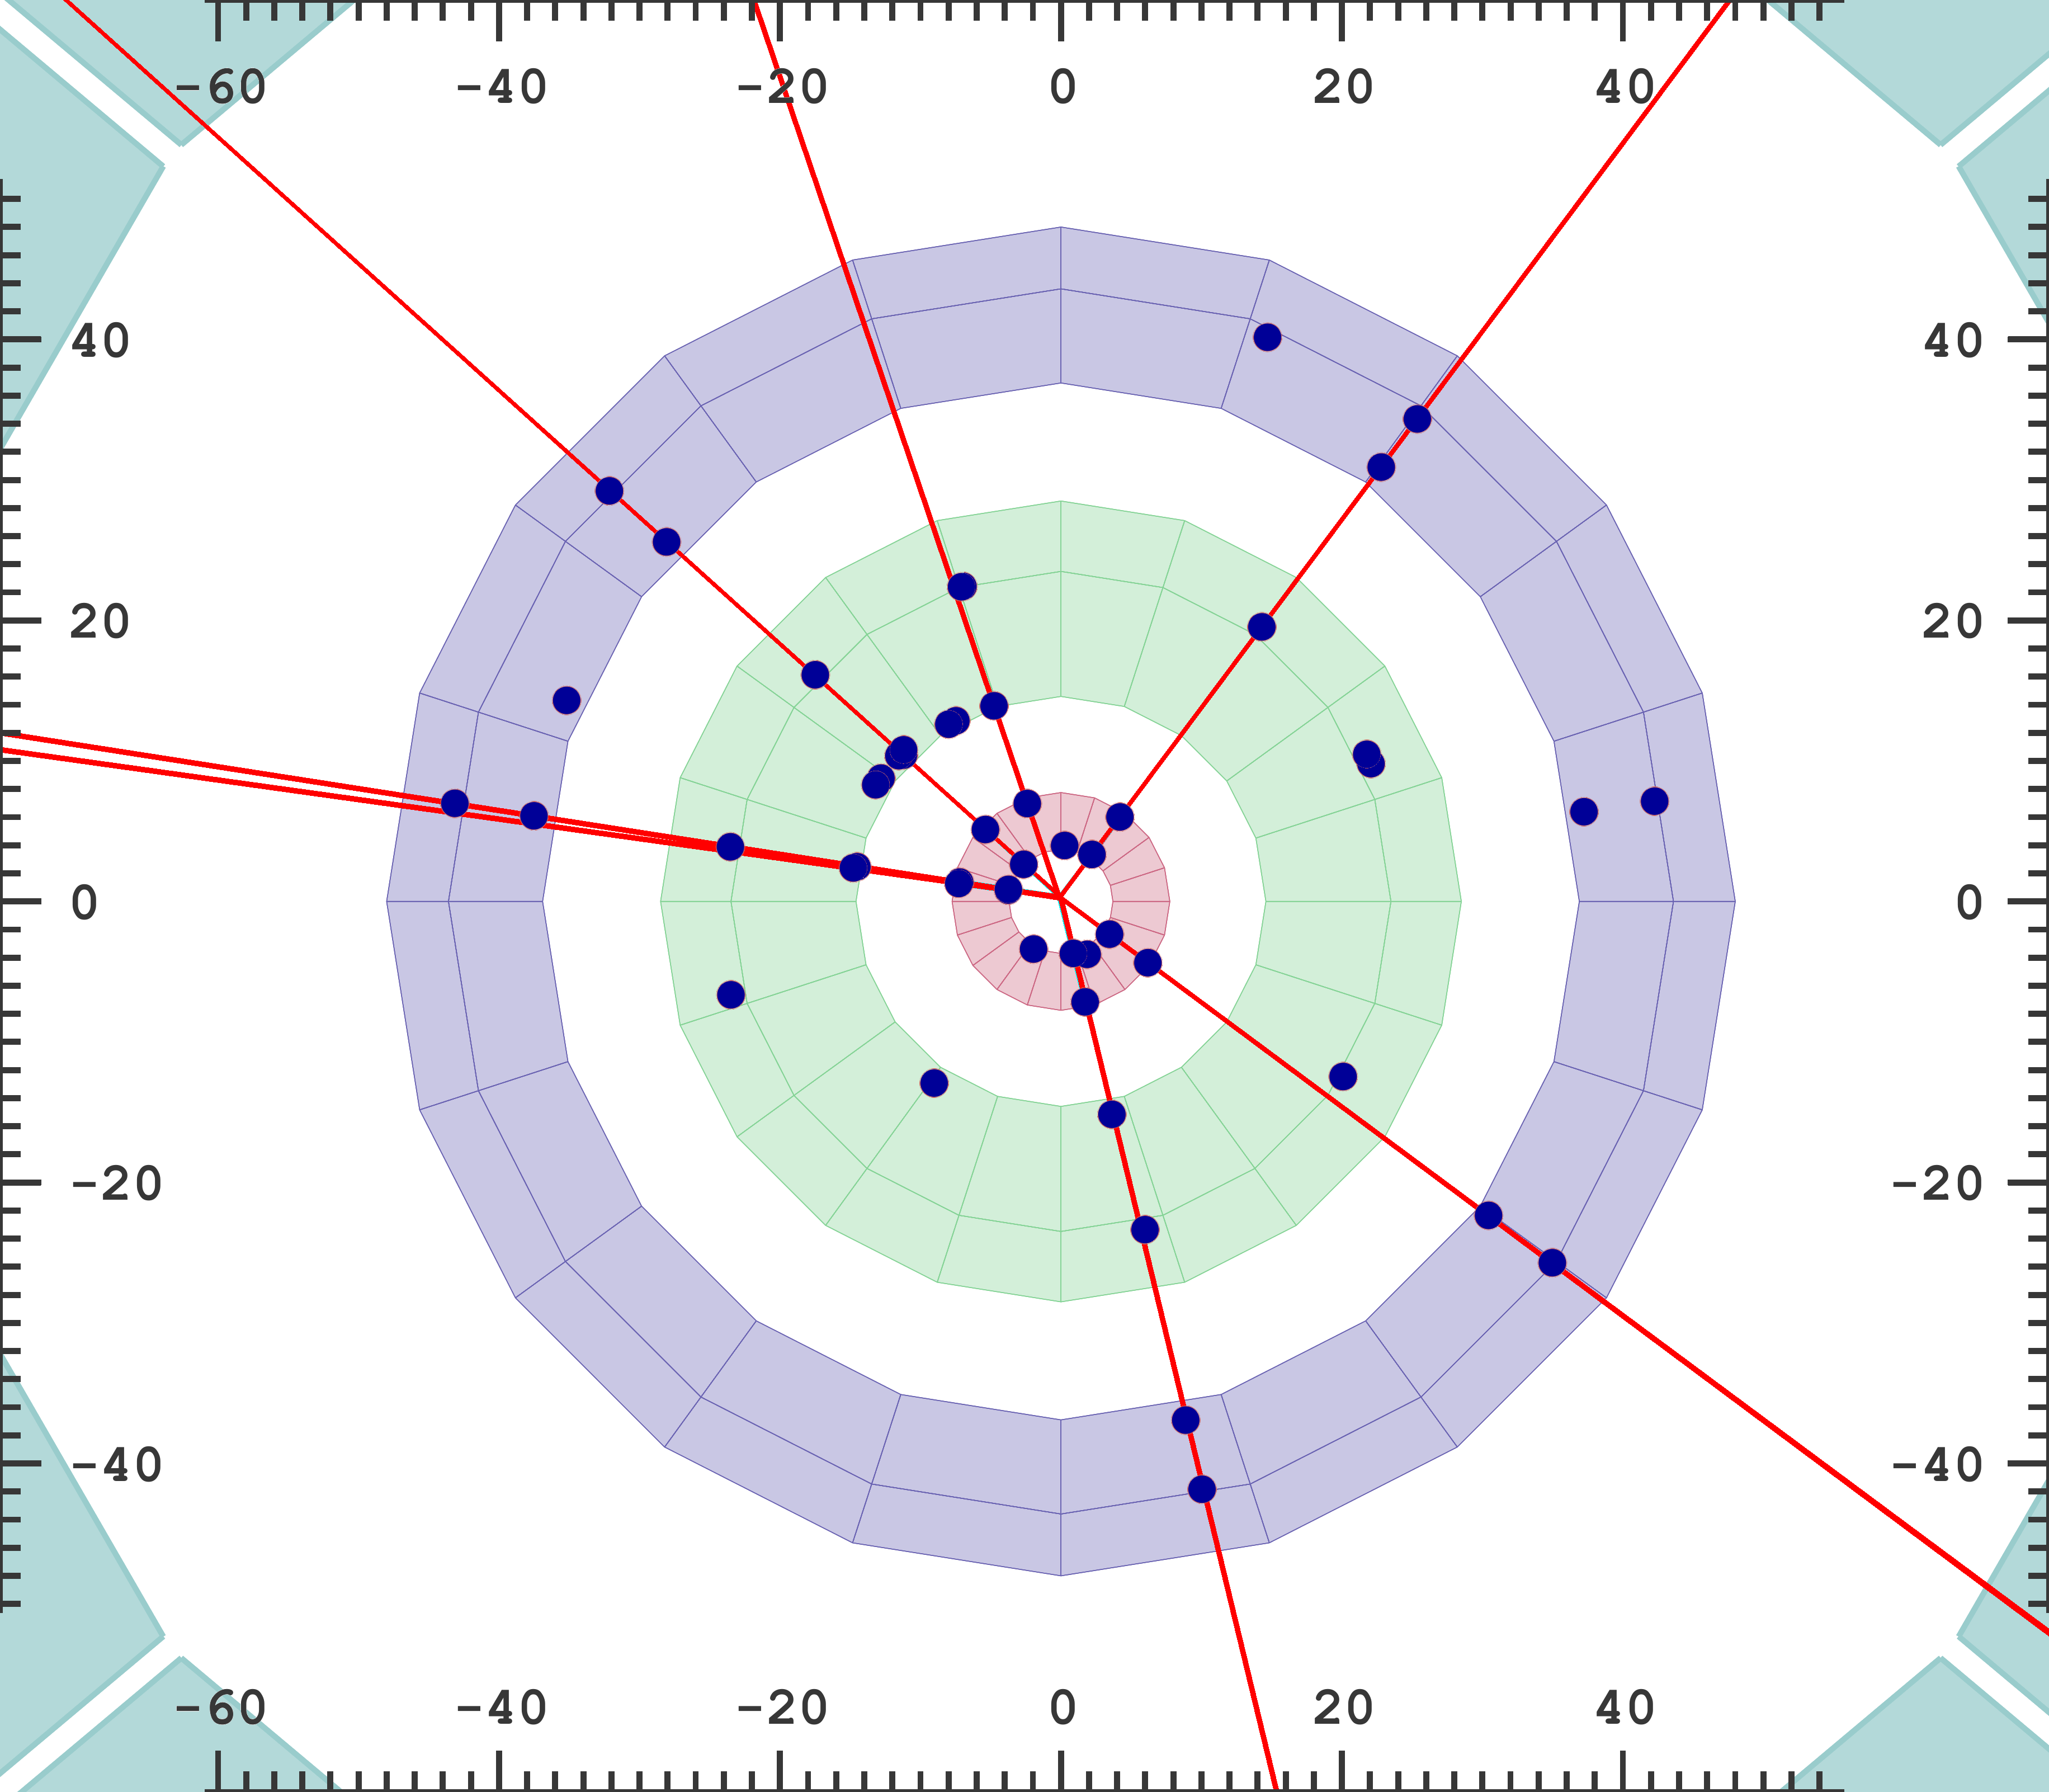
\includegraphics[width=8cm]{chap3/figure/Vertexing/ALICEfirstevent_pPb.png}
  \caption{ITS hits of first proton-proton collision at $\sqrt{s_{NN}}=$900 GeV. The navy points show the hit on ITS and the red lines show the reconstructed tracks~\cite{bib_firstpp}.  }
  \label{fig_3_firstpp}
\end{figure}


Since the readout of SDD and SSD is analog, ITS can provide the information on specific dE/dx in SDD and SSD which follow the Bethe-Bloch formula for each specie and it is used for the particle identification at relatively low momentum particles below 1 GeV/c. 

\subsection{Time Projection Chamber (TPC)}
Time Projection Chamber (TPC) is a large gaseous detector. 
TPC is used as the main tracker in the central barrel of ALICE. 
The specification of TPC is as following, 
\begin{itemize}
\item dE/dx resolution: better than 5\%. \\
\item Relative $p_{T}$ resolution: better than 1\% at $p_{T}=$1 GeV/c and 2.5\% at $p_{T}=$4 GeV/c. \\
\item Two track resolution capability capability of separating tracks with a relative momentum difference $<$ 5 MeV/c.
\end{itemize}
Figure~\ref{fig_3_tpclayout} shows the schematics of TPC.
It consists of large cylindrical gas chamber with 85 cm inner radius and 250 cm outer radius. 
The length is 500 cm along with the z-axis. 
The gas volume is 88 $\rm{m^{3}}$ and filled with $\rm{Ne/CO_{2}}$ or $\rm{Ar/CO_{2}}$.
During Run1, it was filled with $\rm{Ne/CO_{2}}$ (90\%/10\%) mixture gas.
\begin{figure}[!h]
  \centering
  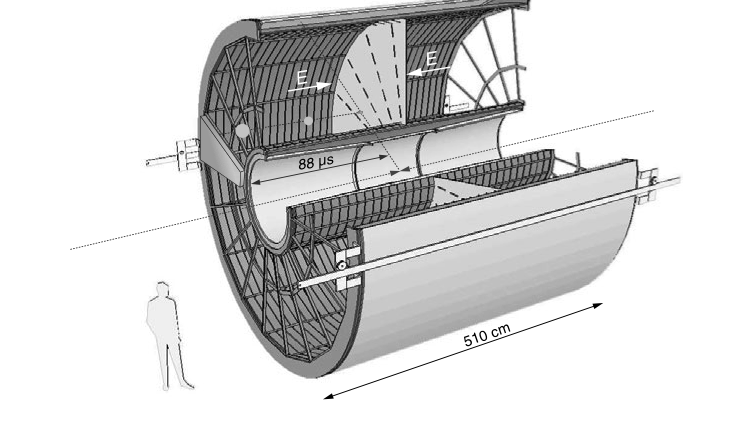
\includegraphics[width=12cm]{chap3/figure/TPC/Schematics_TPC.png}
  \caption{Schematics of TPC layout~\cite{bib_tpctdr}.}
  \label{fig_3_tpclayout}
\end{figure}

The structure of the field cage is also cylindrical to maintain an uniform electric field between the Central Electrode (CE) and both end-planes (A-side and C-side).
In case of $\rm{Ne/CO_{2}}$ mixture gas, the field cage is operated at the drift field$=$400 V/cm with 100 kV at the CE. 
The maximum drift time reaches 90 $\mu$s.
The primary electrons ionized by the interaction of charge particles inside the active volume drift toward the both end-planes of A-side and C-side.
The gating grid of the readout chambers are usually closed and it is opened if TPC accepts L1 trigger signal in 6.5 $\mu$s after a collision.
It prevents from space charges in the drift region due to drifting back of positive ions generated by the multiplication of the readout chamber which cause background signals. 
The signal charges are multiplied by the Multi-Wire Proportional Chambers (MWPCs) with the gain ~7000-8000 as shown in Fig.~\ref{fig_3_tpcchamber}. 
The signals are induced in the pad-planes which have 159 readout pad rows along the perpendicular direction of the beam axis.
\begin{figure}[!h]
  \centering
  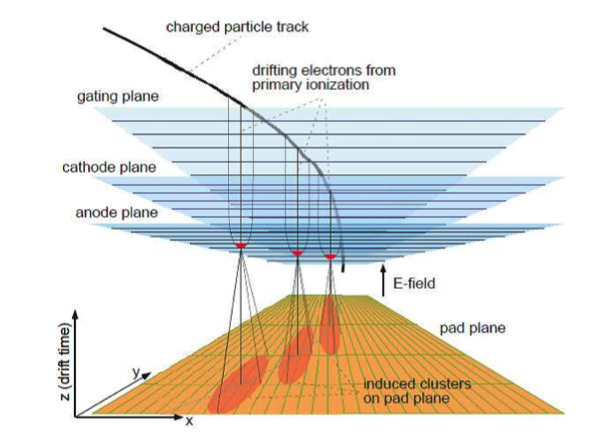
\includegraphics[width=12cm]{chap3/figure/TPC/Schematics_MWPCs.png}
  \caption{Schematics of readout chambers of TPC~\cite{bib_tpctdr}.}
  \label{fig_3_tpcchamber}
\end{figure}
The analog signals shaped with Preamplifier and Shaper (PASA) are digitized by 10-bit pipelined-ADC with 5 MHz sampling~\cite{bib_pasa}. 
They are used for the clustering and provide the 3-D position of specific energy loss by the ionization. 

\subsection{Transition Radiation Detector (TRD)}
\label{sec_3_trd}
The main purpose of the Transition Radiation Detector (TRD) is to give electron identification with good e/$\pi$ separation in wide momentum range and tracking capability of charged particles in the central barrel.
The e/$\pi$ separation reaches to 100 above 1 GeV/c. 
%Figure~\ref{fig_3_5_3} shows the picture of a TRD super module. 

TRD which surrounds TPC covers the full azimuthal acceptance with 18 super modules with the pseudo-rapidity coverage $|\eta| <$ 0.9. 
The super module is divided into 5 stacks along the $\eta$ direction. 
Each stack consists of 6 layers of MWPCs filled with $\rm{Xe/CO_{2}}$ (85\%/15\%) with the radiators (polypropylene fiber mat) for the transition radiation in front of their chambers as shown Fig.~\ref{fig_3_trdlayout}.
In total, 540 chambers(18 super modules in $\phi$ $\times$ 5 stacks in $\eta$ $\times$ 6 layers in r) are installed in principle but during Run1, 13 super modules were installed. 
The lower super modules don't contain the center stack due to the reduction of the material budget in front of PHOS detector. 
\begin{figure}[!h]
  \centering
  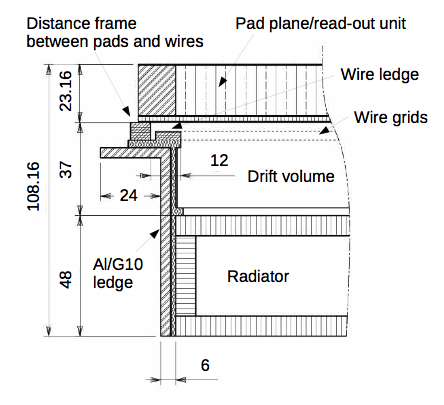
\includegraphics[width=8cm]{chap3/figure/TRD/CrossSection_Chamber.png}
  \caption{The corss section of the structure of TRD chamber\cite{bib_trdtdr}.}
  \label{fig_3_trdlayout}
\end{figure}

%\begin{figure}[!h]
%  \centering
%  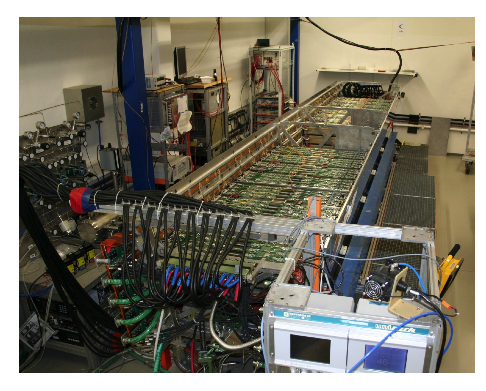
\includegraphics[width=8cm]{chap3/figure/TRD/SuperModules.png}
%  \caption{Super module of TRD during assembly.}
%  \label{fig_3_5_3}
%\end{figure}
%\begin{figure}[!h]
%  \centering
%  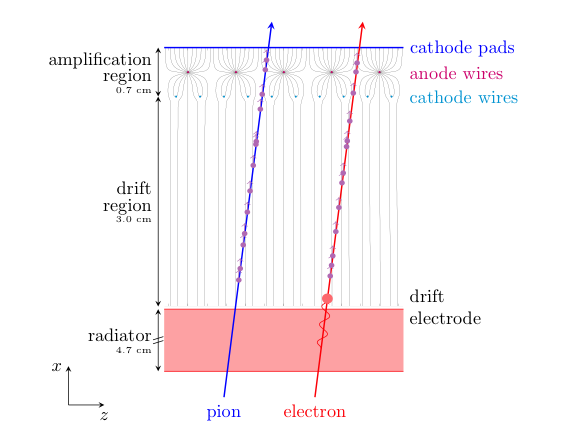
\includegraphics[width=12cm]{chap3/figure/TRD/Schematics_TRDChamber.png}
%  \caption{Schematics of readout chambers of TRD.}
%  \label{fig_3_5_2}
%\end{figure}

Charged particles generated in collisions penetrate into the radiator which has 4.8 cm depth first. 
The condition of the transition radiation in the radiator is, 
\begin{equation}
  \gamma > 800
\end{equation}
At LHC energy, only electrons fulfill this condition, 
Therefore TRD can separate the electrons and pions by detecting the deposited charges of transition radiation photons.
Since Xe has a good absorption length for transition radiation photons ($E_{TR}\sim$ 10 keV) as shown in Fig.~\ref{fig_3_xe}, transition radiation photons are sufficiently absorbed just in front of the radiator. 
\begin{figure}[!h]
  \centering
  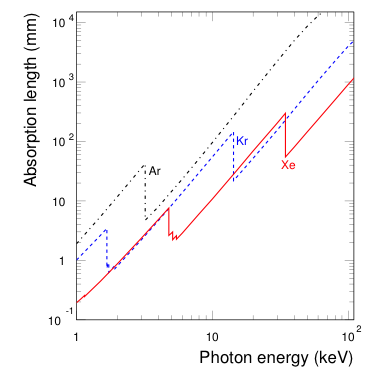
\includegraphics[width=8cm]{chap3/figure/TRD/AbsorptionLength.png}
  \caption{Absorption length for gases~\cite{bib_trdtdr}.}
  \label{fig_3_xe}
\end{figure}

The left panel of Fig.\ref{fig_3_trdschema} shows the schematics of the readout chamber. 
The readout chamber is operated with the drift field$=$700 V/cm and the drift velocity reaches 1.5 cm/$\mu$s.
In this operation, the Lorentz Angle reaches 8 rad in the magnetic field of the L3 magnet. 
The maximum drift length which corresponds to that of transition radiation photons is 3 cm. 
The signals are readout with PASA and TRAP (Tracklets Processor) chip on the Multi-Chip Module (MCM) mounted on the Readout Board (ROB). ROB is located at the back-plane of chambers.%~\cite{bib_trap}.
The operation of the subdetectors is based on the L0, L1, and L2 trigger signals generated from CTP in ALICE for the synchronization and prevention of detector busy as described in Section~\ref{sec_3_trigger}. 
However it is more complicated in case of TRD. 
For the power consumption and noise reduction, the TRAP chips are usually in the low power mode that the front-end ADC is off. 
Therefore a wake-up signal for the electronics is needed but L0 trigger has too long latency from an interaction to cope with the full signal deposited in the TRD chambers. 
\begin{figure}[!h]
 \begin{minipage}{0.5\hsize}
  \begin{center}
  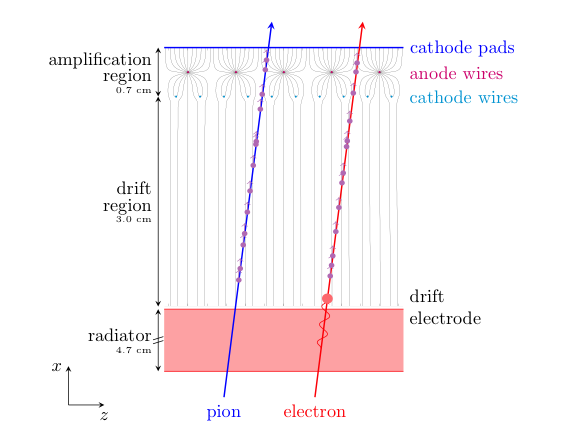
\includegraphics[width=8cm]{chap3/figure/TRD/Schematics_TRDChamber.png}
  \end{center}
 \end{minipage}
 \begin{minipage}{0.5\hsize}
  \begin{center}
  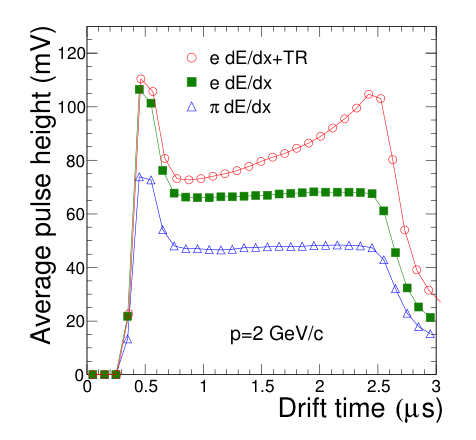
\includegraphics[width=7cm]{chap3/figure/TRD/PulseHeight.png}
  \end{center}
 \end{minipage}
  \caption{Left: Schematics of the readout chamber of TRD. Left: Average pulse height as a function of the drift time for pions and electrons. The signal of transition radiation photons contribute to the latter time bins~\cite{bib_trdtdr}.}
  \label{fig_3_trdschema}
\end{figure}

The wake-up signal is issued by the pretrigger system without the latency of CTP communication.%~\cite{bib_pretrigger}.  
The pretrigger box is placed just under the central ALICE detectors to reduce transport latency (inside the L3 magnet).
It receives L0 inputs from fast detectors, V0, T0, and TOF detectors which are the same signals sent to CTP. 
Therefore in the ideal case for example neglecting detector busy, the same trigger condition is achieved. 
After decision in the pretrigger box, the wake up signal is sent to all TRD sectors and the operation of ADC start to work. 
The later L0 trigger signals from CTP are forwarded to the supermodules via the pretrigger system. 
In p-Pb collisions during Run1, the pretrigger efficiency is about 90\%. 

The sampling frequency of 10-bits ADC in TRAP is 10 MHz and the number of time bins is 22-24.
The right panel of Fig.~\ref{fig_3_trdschema} shows the pulse height for electrons and pions~\cite{bib_trdtdr}. 
The signals contain specific energy loss for each species via ionization and the contribution of transition radiation photons. 
The contribution of transition radiation photons is localized at the latter time bins since they have long drift length. 
The digital filtering for the ADC data like non-linearity, pedestal filter, gain correction, and tail cancellation is done in the MCM.


TRAP chip also has hardware preprocessor and two-stage CPUs for the cluster finding and tracklet reconstruction. 
Therefore TRD has an online tracking capability and provide rare event triggers for electrons and charged jets.
The online track reconstruction of TRD is summarized in Appendix. 
%The online track reconstruction is described in Section.\ref{sec_3_trdonline}. 
%\begin{figure}[!h]
%  \centering
%  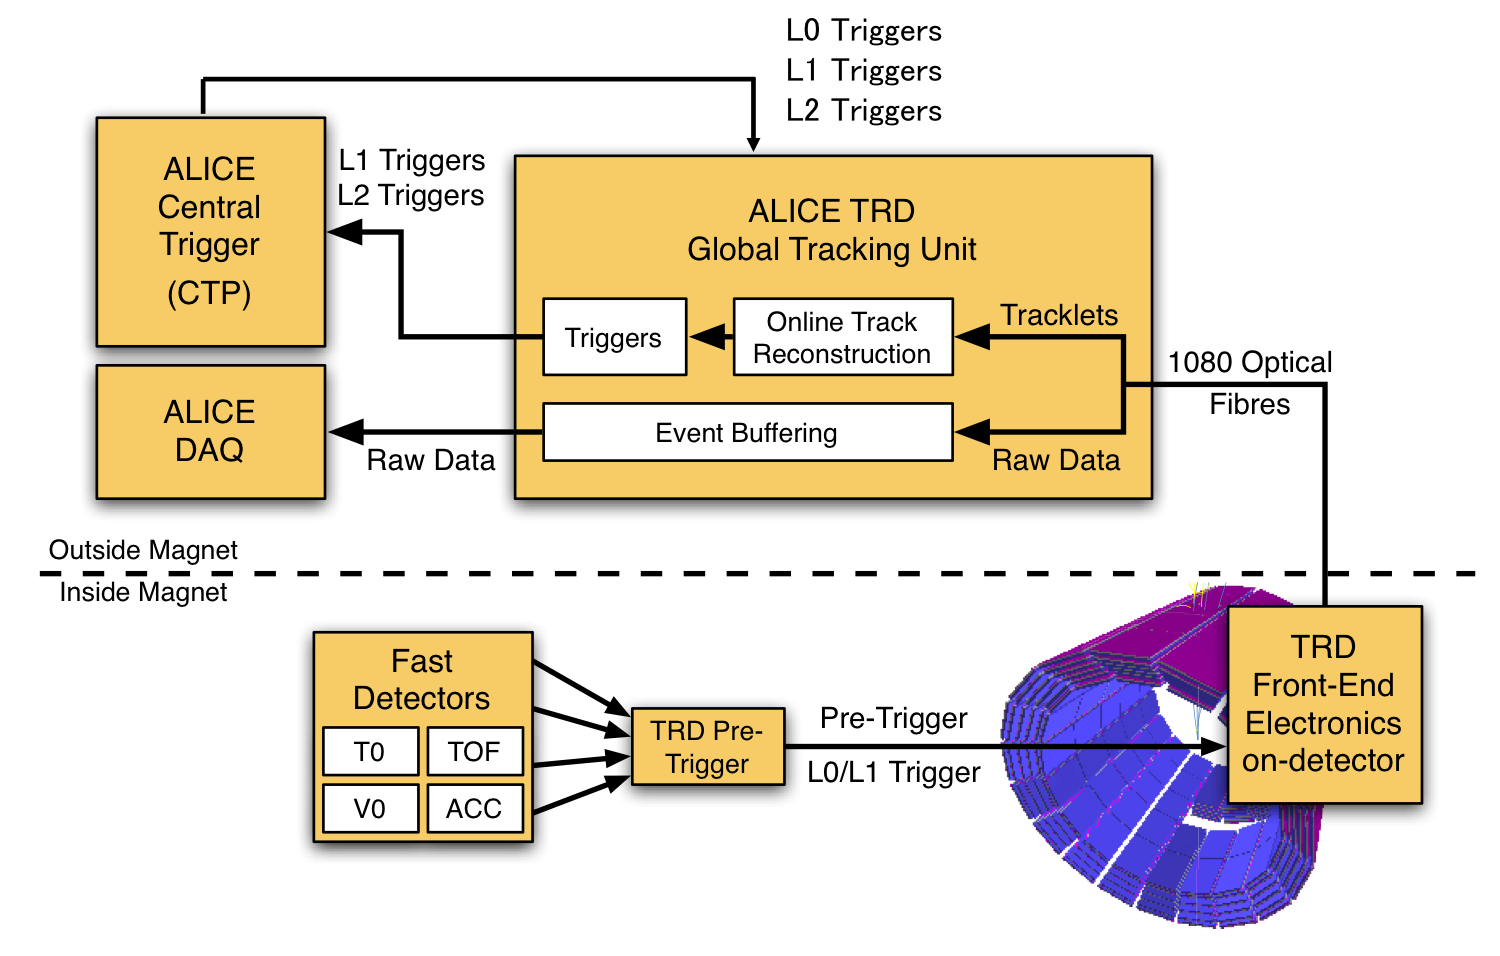
\includegraphics[width=12cm]{chap3/figure/TRD/DataProcess_TRD.png}
%  \caption{Data processing of TRD\cite{bib_trdpaper}.}
%  \label{fig_3_5_5}
%\end{figure}

All raw data and local tracklet data for online event triggers are sent to the Global Tracking Unit (GTU). 
GTU decides to proceed further steps by receiving L0 trigger from CTP. 
And then, if L1 trigger is accepted, the data is transferred to Data Acquisition system (DAQ).

Figures~\ref{fig_3_trdepi} show the performance plots of e/$\pi$ separation using TRD~\cite{bib_aprrun1}.
1DLQ method is using inclusive charge sum for the electron likelihood calculation. 
On the other hand, 2DLQ method is based on the calculation of integrated charge sum dividing former time bins and that for the latter time bins. 
Since the signals of transition radiation localize in the latter time window, better e/$\pi$ separation can be performed compared to 1DLQ method.
%The result of Neural Network using electron and pion samples has potential .  
Figure shows the pion efficiency with 90\% electron efficiency with different methods.
The pion rejection can reach 100 at $p_{T}=$2 GeV/c. 
\begin{figure}[!h]
 \begin{minipage}{0.5\hsize}
  \begin{center}
  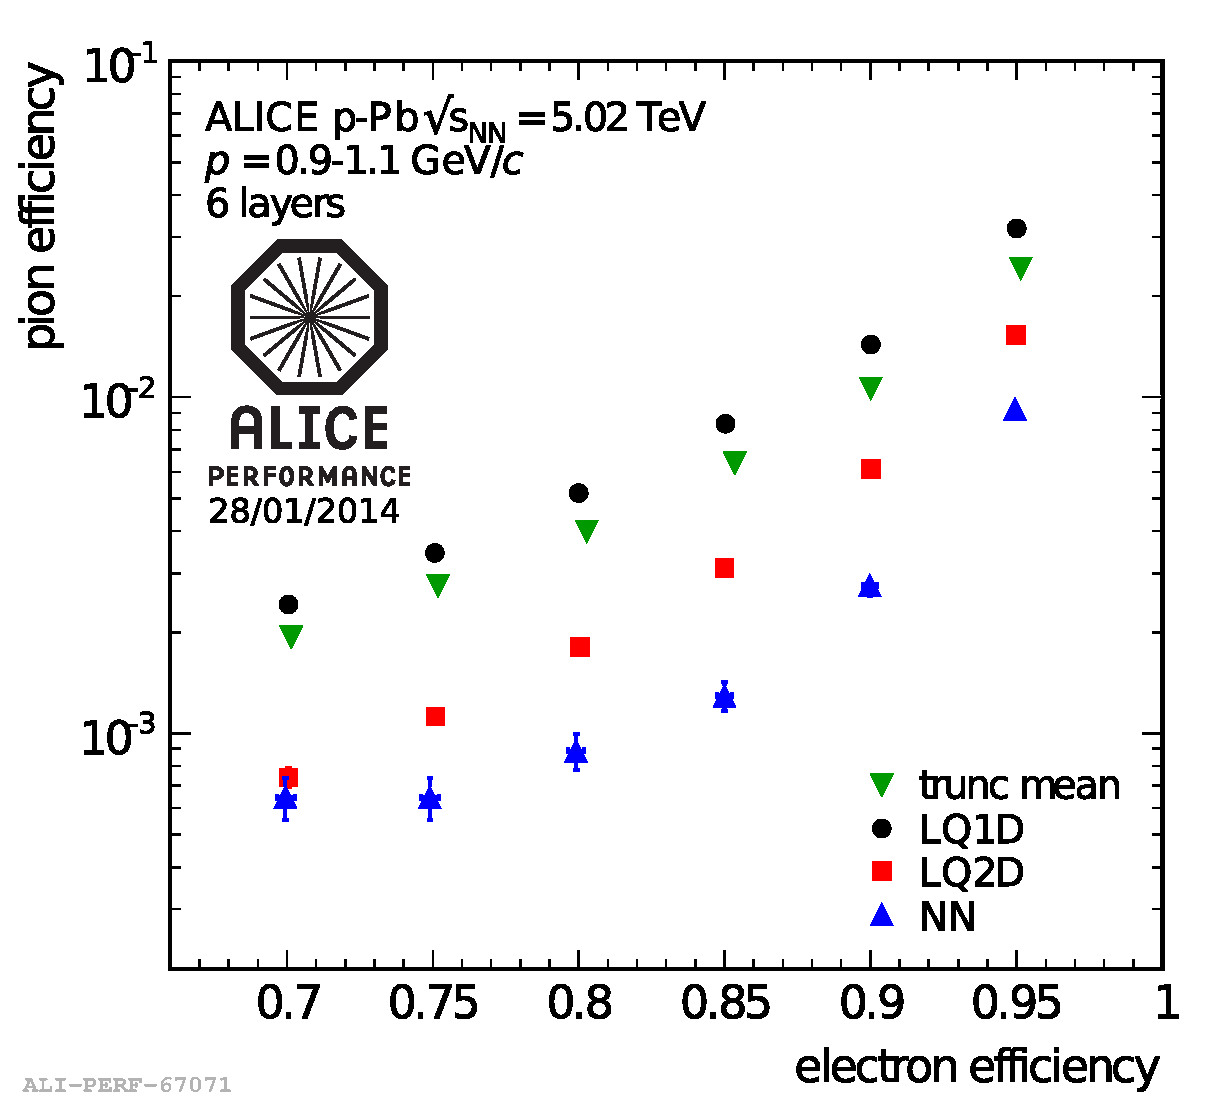
\includegraphics[width=7cm]{chap3/figure/TRD/TRDEleEffvsPiEff.eps}
  \end{center}
  \label{fig_3_trd_1}
 \end{minipage}
 \begin{minipage}{0.5\hsize}
  \begin{center}
  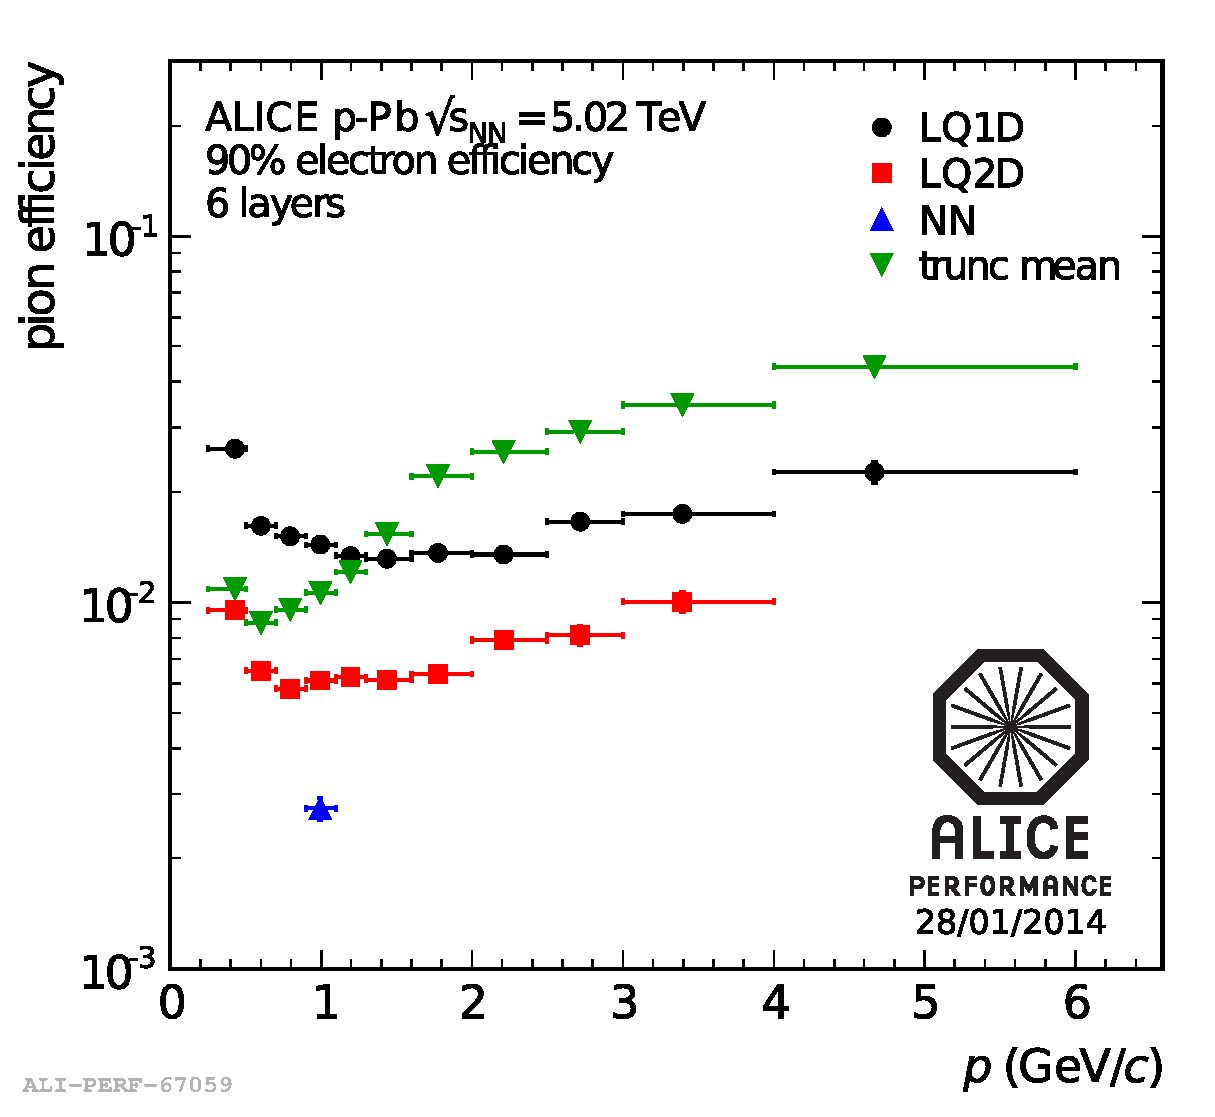
\includegraphics[width=7cm]{chap3/figure/TRD/TRDPionEffvsP_pPb.eps}
  \end{center}
 \end{minipage}
  \caption{Left Panel: Electron Efficiency vs Pion Efficiency with TRD PID in p-Pb collision at $\sqrt{s_{NN}}=$5.02 TeV. Right Panel:Pion Efficiency at the electron efficiency $=$ 90 \% with TRD PID as a function of transverse momentum in p-Pb collision at $\sqrt{s_{NN}}=$5.02 TeV~\cite{bib_aprrun1}
.
}
  \label{fig_3_trdepi}
\end{figure}


\subsection{Time-Of-Flight detector (TOF)}
Time-Of-Flight detector (TOF) is used for the particle identification of pions, kaons, protons, and electrons at $p_{T} <$ 3.0 GeV/c.
Figure~\ref{fig_3_toflayout} shows the layout of TOF. 
It is located at radius of 3.8 m and covers the full azimuthal and $|\eta| < $ 0.9 acceptance with 18 super modules in $\phi$. 
\begin{figure}[!h]
  %\begin{minipage}{0.5\hsize}
    \begin{center}
      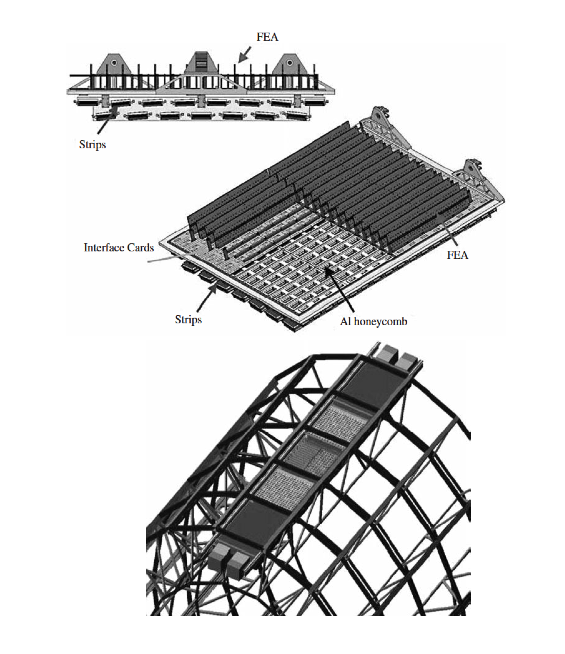
\includegraphics[width=10cm]{chap3/figure/TOF/SuperModule_TOF.eps}
    \end{center}
  %\end{minipage}
    \caption{Schematics of Super modules of TOF and detail of one TOF module of aluminium honeycomb plane~\cite{bib_toftdr}.}
    \label{fig_3_toflayout}
\end{figure}

Figure~\ref{fig_3_tofmrpc} shows the schematics of MRPCs for TOF. 
TOF consists of an array of Multi-gap Resistive Plate Chamber (MRPCs). 
The chamber is divided into two stack on each side of the central anode. 
Each stack has five gas gaps of 250 $\mu$m to keep high and uniform electric field. 
  %\begin{minipage}{0.5\hsize}
\begin{figure}
    \begin{center}
      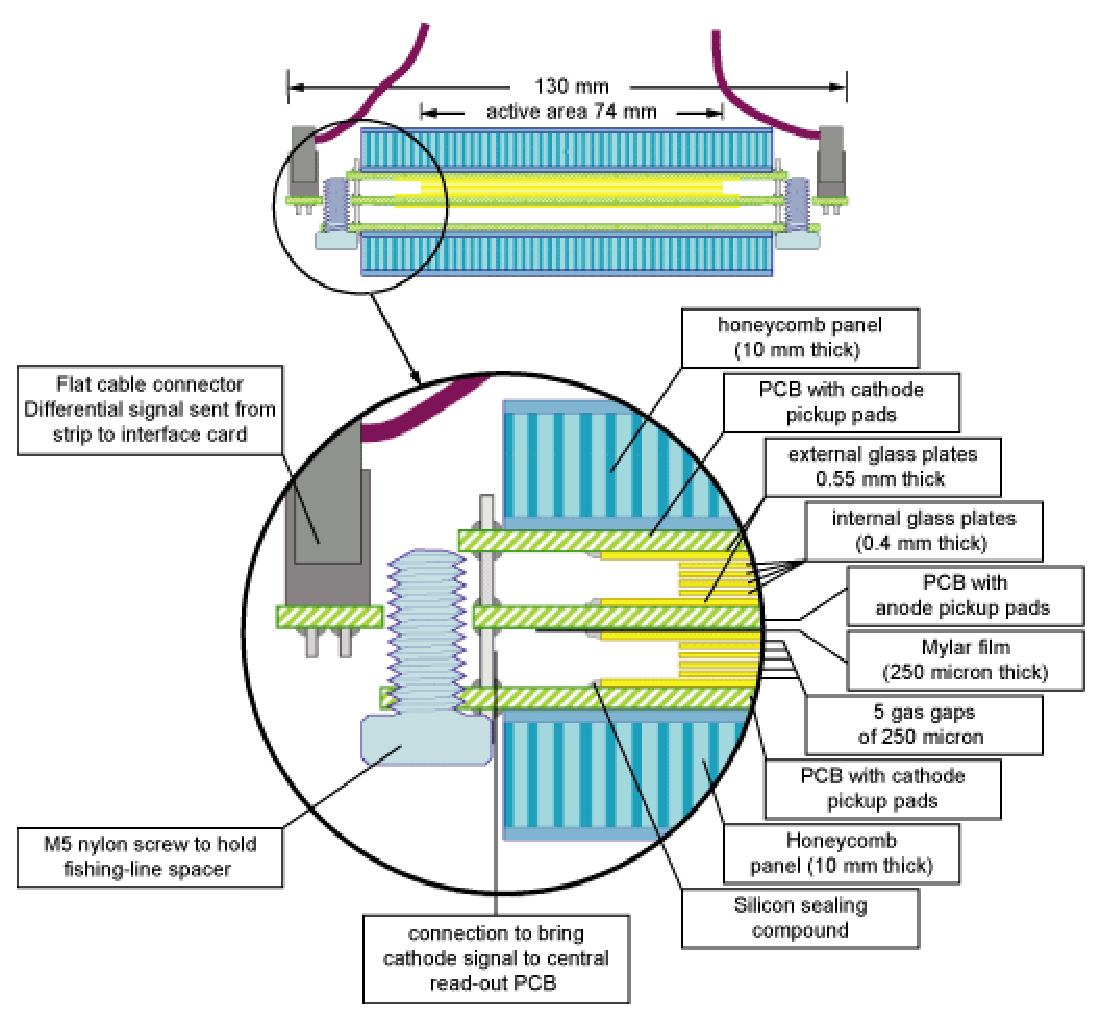
\includegraphics[width=8cm]{chap3/figure/TOF/TOFMRPC.eps}
    \end{center}
  %\end{minipage}
  \caption{ 
    Schematics of MRPCs for TOF~\cite{bib_toftdr}.
  }
  \label{fig_3_tofmrpc}
\end{figure}
When charged particles transverse the chambers, avalanche of electrons are produced immediately. 
The avalanche electrons are readout with pad of 2.5$\times$3.5 $cm^{2}$ arranged in 2 rows.
The time resolution of TOF itself achieves 40 ps. 
The start time of Time-Of-Flight is determined by the T0 detector.
Considering other uncertainties, the arrival time of charged particles can be measured with less than 100 ps resolution. 

Combined with momentum measurement, the relative velocity which is proportional to arrival time at TOF for each species distribute with the following relationship, 
\begin{equation}
  \beta = \frac{p}{m_{0}\gamma c}
\end{equation}

In addition, TOF also contribute to the pretrigger for TRD wake-up. 

\section{Vertexing}
\label{sec_3_vtx}
Primary vertex which is thought as the collision vertex is performed by two steps. 
First estimation of primary vertex which is thought as the collision vertex is performed by the hits on SPD detectors.
The pairs of SPD hits in each two layer which have close azimuthal angle are selected as tracklets.
Tracklets have to across the cylindrical fiducial region. 
Fiducial cuts for tracklets selection are optimized in each collision system with respect to the efficiency and background contamination.
Tracklets are selected within DCA between pair of tracklets $<$ 1 mm. 
For all tracklets, the following value is calculated,  
\begin{equation}
  d_{i} = \Sigma \frac{x_{i}-x_{0}}{\sigma_{x_{i}}}
\end{equation}
where $x_{0}$ is the expected 3-D position of the vertex, $x_{i}$ $\sigma_{x_{i}}$ is the 3-D position and the resolution of the tracklets. 
The position of the primary vertex with SPD is determined from minimum D = $\Sigma d_{i}^{2}$. 
This routine is done twice with two (loose/tight) cut setting on fiducial region and $\Delta\phi $. 
SPD is operated in the magnetic field but the effect can be negligible because of the small radius.
This vertex is used for track reconstruction. 

The final determination of primary vertex is recalculated with reconstructed tracks using ITS and TPC.  
The 3-D position of primary vertex is calculated using central between selected track pairs. 
These positions are determined as the position of the closest approach of the two tracks.  

Figure~\ref{fig_3_vtxperformance} show the finding efficiency and the position resolution of the primary vertex reconstruction with reconstructed tracks as a function of the charged particle multiplicity. 
\begin{figure}[!h]
  \begin{minipage}{0.5\hsize}
    \begin{center}
      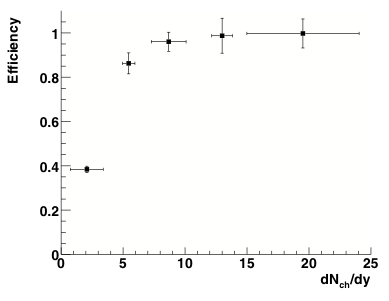
\includegraphics[width=8cm]{chap3/figure/Vertexing/Efficiency_Vtx.png}
    \end{center}
  \end{minipage}
  \begin{minipage}{0.5\hsize}
    \begin{center}
      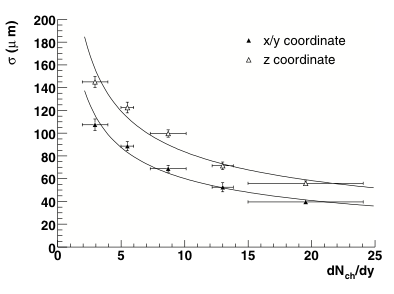
\includegraphics[width=8cm]{chap3/figure/Vertexing/Resolution_Vtx.png}
    \end{center}
  \end{minipage}
  \caption{ 
    Efficiency (Left) and position resolution (Right) of the primary vertex with 3-D method in case of pp collisions~\cite{bib_vtxreso}.  
  }
  \label{fig_3_vtxperformance}
\end{figure}

\section{Tracking System of Charged Particles with the ALICE Detectors}
\label{sec_3_trackrec}
\begin{figure}[!h]
  \centering
  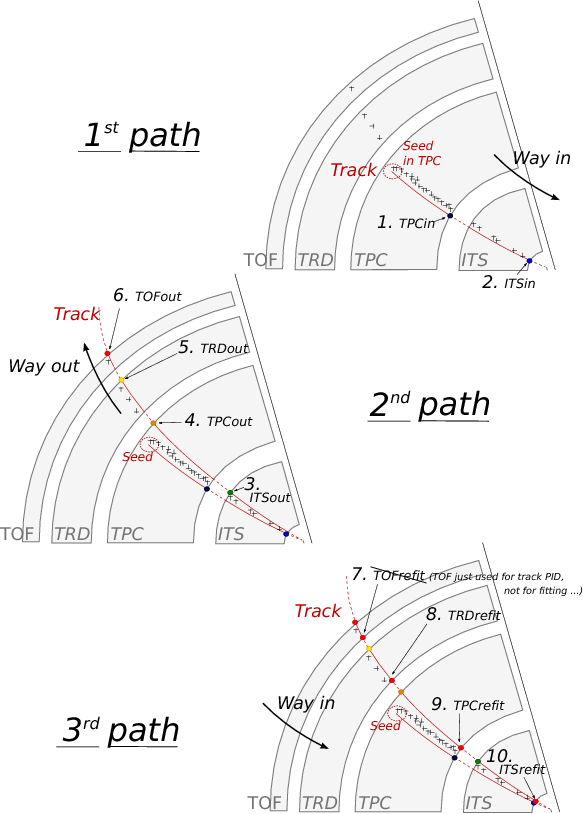
\includegraphics[width=7cm]{chap3/figure/TrackReconstruction/Schematics_TrackingALICE.png}
  \caption{Principles of tracking for an ALICE event, showing the three successive paths allowing to build a track and refine its parameters. Numbers ranging from 1 to 10 mention the bits that are activated in case of success during the propagation of the Kalman filter at the considered stage~\cite{bib_schematrackrec}.}
  \label{fig_3_trackrec}
\end{figure}
Track reconstruction in the central barrel is performed using clusters found in each detector along the trajectory of charged particles. 
The track reconstruction follows three steps as shown Fig.~\ref{fig_3_trackrec}. 
%The start point of tracking is determined by the TPC clusters induced by ionization along the trajectory of charge particles.
The start point of tracking is determined by the most outer cluster in the TPC where the track density is relatively lower than inner detectors. 
TPC provides 159 clusters which are reconstructed from 2-dimensional information on pad-plane-time. 
Track is fitted using Kalman-Filter algorithm inward. 
The track state vector is chosen as 
\begin{equation}
  x^{T} = (y, z, C, tan\lambda, \eta)
\end{equation}
where y, z are local position in the TPC, C is coverture and $\lambda$ is dip angle between the track and padplane as shown Fig.~\ref{fig_3_tpclocalcood}. 
\begin{figure}[!h]
  \centering
  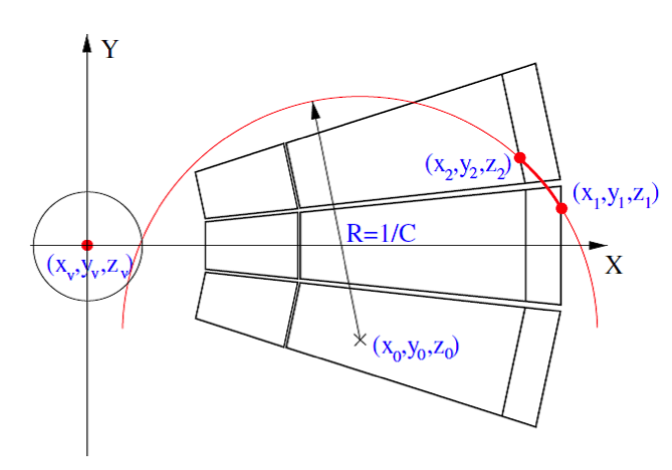
\includegraphics[width=7cm]{chap3/figure/TrackReconstruction/TPCLocalCoodinate.png}
  \caption{Local coordinate system for one sector of TPC.}
  \label{fig_3_tpclocalcood}
\end{figure}
This process is done from high momentum candidate because these tracks can be found more precisely compared to low momentum tracks. 
After propagation to the most inner ITS layer, the propagation is done again from ITS to TPC using Kalman-Filter. 
This propagation also include the hits of TRD, TOF, and EMCAL. 
Finally, the propagation called 'refit' is done from outward to ITS for the determination of the track position. 



Figure~\ref{fig_3_trackeff} shows the TPC track finding efficiency in pp and Pb-Pb collisions~\cite{bib_aprrun1}. 
There is a consistency between the reconstruction efficiency in pp and Pb-Pb collisions. 
It implies that the reconstruction efficiency is not affected by the charged particle multiplicity due to high granularity of the detectors.  
\begin{figure}[!h]
  \centering
  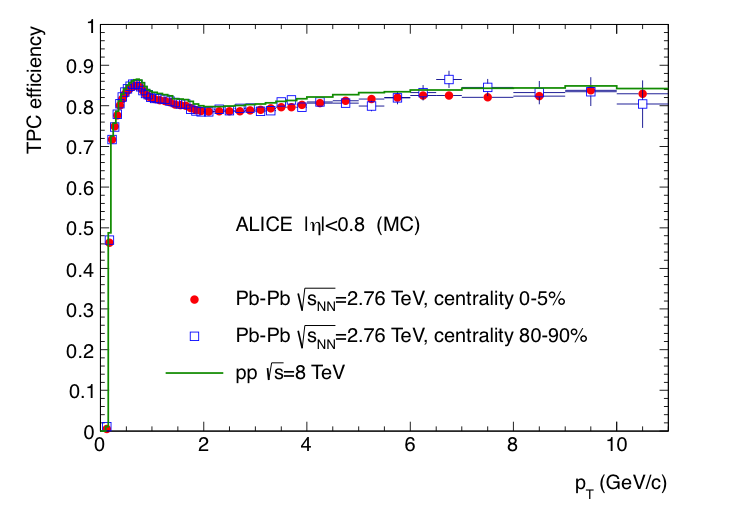
\includegraphics[width=10cm]{chap3/figure/TrackReconstruction/TrackEff.png}
  \caption{TPC track finding efficiency in pp and Pb-Pb collisions~\cite{bib_aprrun1}.}
  \label{fig_3_trackeff}
\end{figure}

Figure~\ref{fig_3_momreso} shows the transverse momentum resolution in p-Pb collisions~\cite{bib_aprrun1}.
The y-axis is defined as following, 
\begin{equation}
  \frac{\sigma_{p_{T}}}{p_{T}} = p_{T}\sigma_{1/p_{T}}.
\end{equation}
With ITS hits, the momentum resolution can be improve significantly. 
The impact parameter of reconstructed tracks can also be determined precisely using ITS. % that enables to separate charm and bottom contribution. 
\begin{figure}[!h]
  \centering
  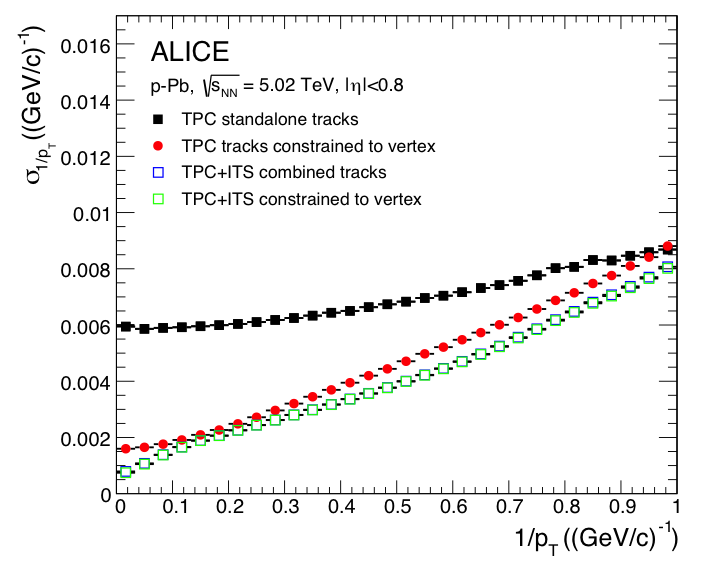
\includegraphics[width=10cm]{chap3/figure/TrackReconstruction/MomReso_pPb.png}
  \caption{Inverse momentum resolution in p-Pb collisions at $\sqrt{s_{NN}}=$5.02 TeV~\cite{bib_aprrun1}.}
  \label{fig_3_momreso}
\end{figure}


\section{Particle Identification in ALICE}
\label{sec_3_pid}
ALICE uses various detectors and techniques in wide momentum range to identify particle species. 
The main technique of the particle identification is specific energy loss (dE/dx) of charged particles deposited in the detectors such as ITS, TPC and TRD.
The mean deposited energy loss in detectors can be described by the Bethe-Bloch formula.
\begin{equation}
  -\langle \frac{dE}{dx}\rangle = \frac{4\pi}{m_{e}c^{2}} \frac{nz^{2}}{\beta^{2}} ( \frac{e^{2}}{4\pi\epsilon_{0}} )^{2} [ ln( \frac{2m_{e}c^{2}\beta^{2}}{I(1-\beta^{2})} ) - \beta^{2} ]
\end{equation}
where $e$ is the elementary charge, $m_{e}$ is the electron mass, $n$ is the number density of electrons in the traget material, $z$ is the charge of the particle, and $I$ is the average ionisation potential of the target atom. 

TOF is useful to separate proton and kaon up to 4 GeV/c by measuring the flight time of particles. 
EMCAL also detects electron and photon with their deposited energy. 
%For the high $p_{T}$ particle identification, HMPID can be used. 
However they are not used in this analysis due to the limited acceptance and low reconstruction efficiency. 

\subsection{TPC PID}
The key information for the particle identification in ALICE is TPC dE/dx. 
Figure~\ref{fig_3_tpcpid} shows the deposited energy in TPC (dE/dx) as a function of reconstructed momentum in p-Pb collisions~\cite{bib_aprrun1}.
\begin{figure}[!h]
  \centering
  \includegraphics[width=10cm]{chap3/figure/PID/TPCdEdx_p_pPb.eps}
  \caption{TPC dE/dx vs reconstructed momentum in p-Pb collision at $\sqrt{s_{NN}}=$5.02 TeV~\cite{bib_aprrun1}.}
  \label{fig_3_tpcpid}
\end{figure}
Since the probability of energy loss in TPC follows the Landau distribution, the measured raw TPC signals have long tail at higher side.
In order to reduce the Landau fluctuation of TPC dE/dx for better performance of particle separation, the truncated means of all TPC clusters in the tracks are taken as the value of TPC PID.
The average fraction of truncation is about 20-30\%.  
The truncated mean of TPC dE/dx can be approximated to the gaussian and the resolution reaches up to 5\% for cosmic ray as shown in Fig.~\ref{fig_3_tpcpidreso}~\cite{bib_tpcreso}. 
%The typical PID resolution is about 5-8\%.
\begin{figure}[!h]
  \centering
  \includegraphics[width=10cm]{chap3/figure/TPC/TPCdEdx_resolution.png}
  \caption{TPC dE/dx resolution with cosmic rays as a function the number of TPC hits~\cite{bib_tpcreso}. }
  \label{fig_3_tpcpidreso}
\end{figure}

\section{Trigger System in ALICE}
\label{sec_3_trigger}
All communication on trigger information between subsystems is done via Central Trigger Processor (CTP) with TTC protocol~\cite{bib_ctp,bib_ttc}.
Figure~\ref{fig_3_ctp} shows the block diagram of CTP~\cite{bib_ctp}. 
CTP provides the trigger information and LHC timing signal (BC and Orbit) to subdetectors and also accept trigger signal from subdetectors.  

The trigger scheme in ALICE consists of 3 steps called as Level-0 (L0), Level-1 (L1), Level-2 (L2) trigger, respectively.
Level-0 trigger is mainly used for minimum bias event trigger and the initial activation of some subdetectors. 
L0 trigger inputs from fast subdetectors like V0, T0, EMCAL, and Muon detector are delivered into CTP within 900 ns after a collision. 
It is issued by the L0 processor in CTP, and then L0 accept signal is sent to subdetectors after 1.2 $\mu$s after a collision, 
If L0 is not accepted, all components become ready for the next L0 event. 

The purpose of Level-1 trigger is rare event detection. 
If each subdetector which contributes to L1 trigger receives L0 accept signal, a calculation for L1 issue is performed and L1 contribution is sent to CTP.  
It is issued after 6.5 $\mu$s from an interaction.
If L1 trigger is accepted, raw data of subsystem is transferred to the multi event buffers. 

Level-2 trigger is issued about 100 $\mu$s after the decision of L0 trigger which is determined by the drift time of TPC. 
If L2 trigger is issued, the data is transferred from the event buffers in each subdetectors to (DAQ). 

\begin{figure}[!h]
  \centering
  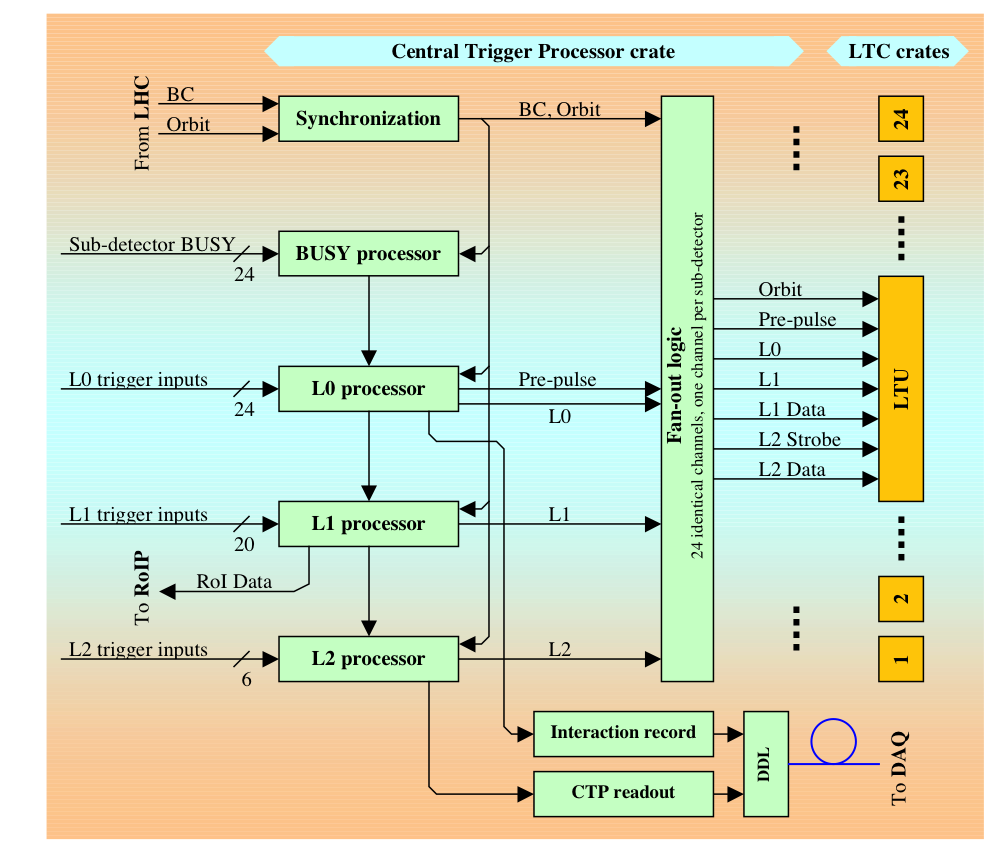
\includegraphics[width=10cm]{chap3/figure/Trigger/CTP.png}
  \caption{Block diagram of CTP~\cite{bib_ctp}.}
  \label{fig_3_ctp}
\end{figure}

%\section{Online Electron Triggers with TRD}
%\label{sec_3_trdonline}
%The online reconstruction of TRD are following. 
%%1. local clustering
%Cluster finding in each chamber is performed by the hardware preprocessor in TRAP chip with two dimensional ADC information of pad rows and time bins. 
%Figure~\ref{fig_3_10_localclustering} shows an example of cluster finding and tracklet reconstruction. 
%The position of clusters is calculated as the center of gravity for each time bin.
%Tracklets are reconstructed by straight line fit for clusters. 
%Tracklets contain 32-bit word information on local position in TRD, deflection, and PID. 
%The data of tracklets are then sent to GTU with 1080 optical fibers after 4.5 $\mu$s after a collision. 
%\begin{figure}[!h]
%  \centering
%  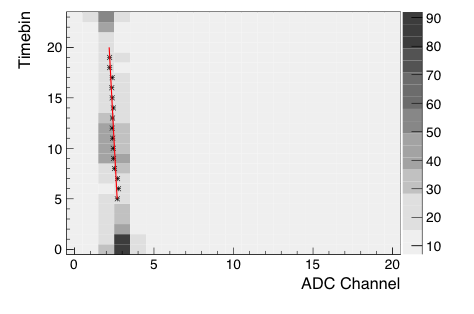
\includegraphics[width=10cm]{chap3/figure/Online/LocalClustering.png}
%  \caption{Cluster finding and tracklets reconstruction in MCM~\cite{bib_trdonline}.}
%  \label{fig_3_10_localclustering}
%\end{figure}


%Global tracking is divided into 2 parts, track matching and track reconstruction. 
%It operates in parallel on subsets of the tracklets which are compatible with a track in the x-z plane, i.e. groups of tracklets which fall into roads pointing to the nominal primary vertex. 
%These are propagated to a plane.
%Tracklets which are close enough on this plane are considered to belong to the same track. 
%The algorithm exploits a fixed read-out order of the tracklets to reduce the number of tracklet combinations which have to compared. 
%In this way, a linear scaling of the tracking time with the number of tracklets is achieved.

%Only selected tracks are reconstructed by the straight line fit as shown in Fig.~\ref{fig_3_10_globaltracking}. 
%The transverse offset from the nominal vertex position is used to estimate the transverse momentum (a $\propto$ 1/$p_{T}$).
%\begin{figure}[!h]
%  \centering
%  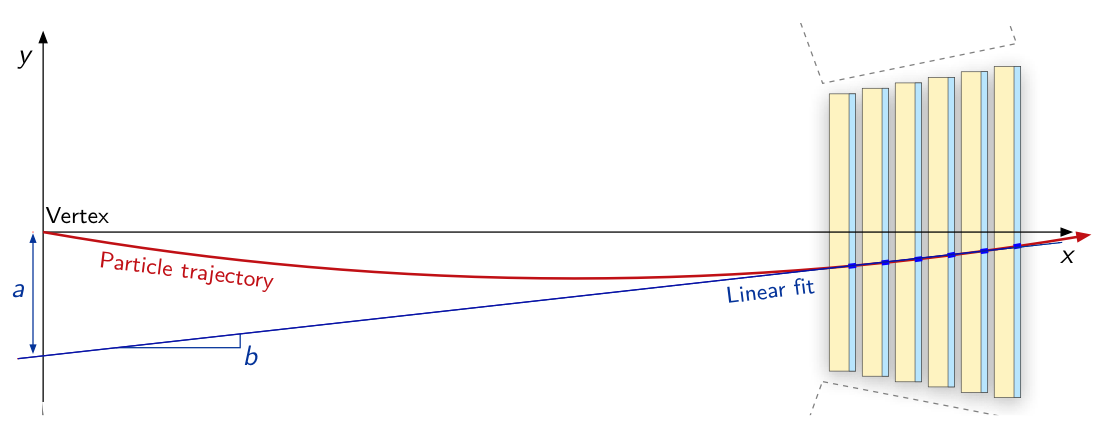
\includegraphics[width=12cm]{chap3/figure/Online/GrobalTracking.png}
%  \caption{Schematics of global tracking in the TRD stack with GTU.}
%  \label{fig_3_10_globaltracking}
%\end{figure}

%Figure\ref{fig_3_10_momreso} shows the online momentum resolution of TRD. 
%The typical value of the resolution is better than 10 \%.
%\begin{figure}[!h]
%  \centering
%  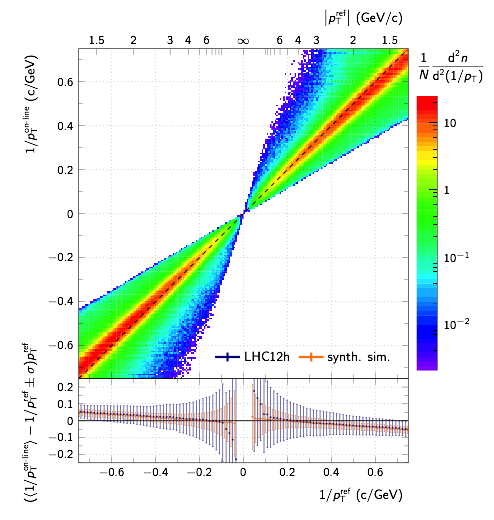
\includegraphics[width=10cm]{chap3/figure/Online/onlinemomreso.png}
%  \caption{Online momentum resolution of TRD.}
%  \label{fig_3_10_momreso}
%\end{figure}

%\begin{figure}[!h]
%  \begin{minipage}{0.5\hsize}
%    \begin{center}
%      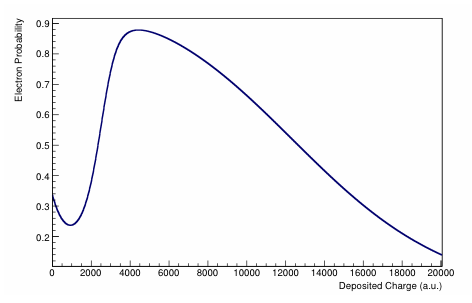
\includegraphics[width=8cm]{chap3/figure/Online/LookUpTable.png}
%    \end{center}
%  \end{minipage}
%  \begin{minipage}{0.5\hsize}
%    \begin{center}
%      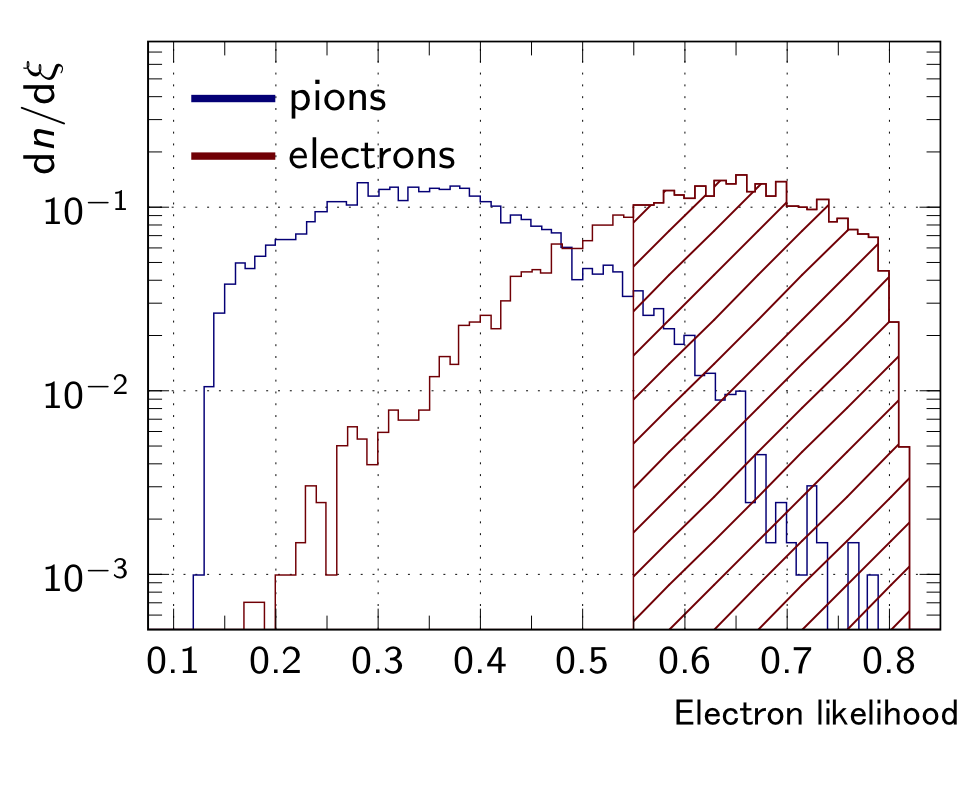
\includegraphics[width=8cm]{chap3/figure/Online/likelihood.png}
%    \end{center}
%  \end{minipage}
%  \caption{ 
%    Left: Lookup table for online electron identification of TRD. Right: Electron likelihood distribution for electrons and pions. 
%  }
%  \label{fig_3_10_elepid}
%\end{figure}
%The left panel of Fig.~\ref{fig_3_10_elepid} shows the lookup table for the online electron identification. 
%The look up table is generated from measured electron and pion samples. 
%The electron likelihood is calculated with 1-D deposited charge sum. 
%The PID value of online tracks is determined by the average of tracklet PID. 

%The right panel of Fig.~\ref{fig_3_10_elepid} shows the electron likelihood distribution for electrons and pions using the lookup tables. 
%TRD provide the 2 different electron triggers during Run1 p-Pb periods as show in Table.~\ref{table_3_10_trigger}. 
%Both triggers require the hit on the first layer of TRD to reduce the contribution of conversion electrons. 
%During Run1, 13 out of 18 super modules of TRD were installed. 
%\begin{table}
%  \centering
% \begin{tabular}{cccc} \hline
%   Trigger & Online $p_{T}(GeV/c)$  & PID (Electron Likelihood) & Layers \\ \hline
%   Heavy Flavor Single Electron & $\geq$3 & $\geq$0.56 & $\geq$5 \\
%    Quarkonia & $\geq$2 & $\geq$0.64 & $\geq$5 \\ \hline
%  \end{tabular}
%  \caption{Electron triggers with TRD during Run1.}
%  \label{table_3_10_trigger}
%\end{table}


\section{Run Condition and Data Set}
\label{sec_3_runcondition}
ALICE took p-Pb collision data in 2 conditions, 'p-Pb' and 'Pb-p'.
p-Pb collisions are defined as a collision traveling Pb from C-side. 
On the other hand, Pb-p collisions are defined that Pb is delivered from A-side. 
Due to the asymmetric energy of colliding protons (4 TeV) and leads (1.58 TeV), rapidity of Center-of-Mass is slightly shifted in the direction of Pb-going ($\sim 0.465$).
%The maximum manageable interaction rate of ALICE is 200 kHz and it corresponds to $10^{29}~s^{-1}\rm{cm}^{-2}$.

Table~\ref{table_3_runcondition} shows the run condition in p-Pb collisions. 
Figure\ref{fig_3_luminosity} shows the integrated luminosity of p-Pb collision during Run1~\cite{bib_aprrun1}. 
The integrated luminosity of the TRD triggered data in $p$-Pb collisions is 1.4 $\rm{nb^{-1}}$.
It corresponds to 20 times larger statistics than the current minimum bias data (0.067 $\rm{nb^{-1}}$).

\begin{figure}[!h]
  \centering
  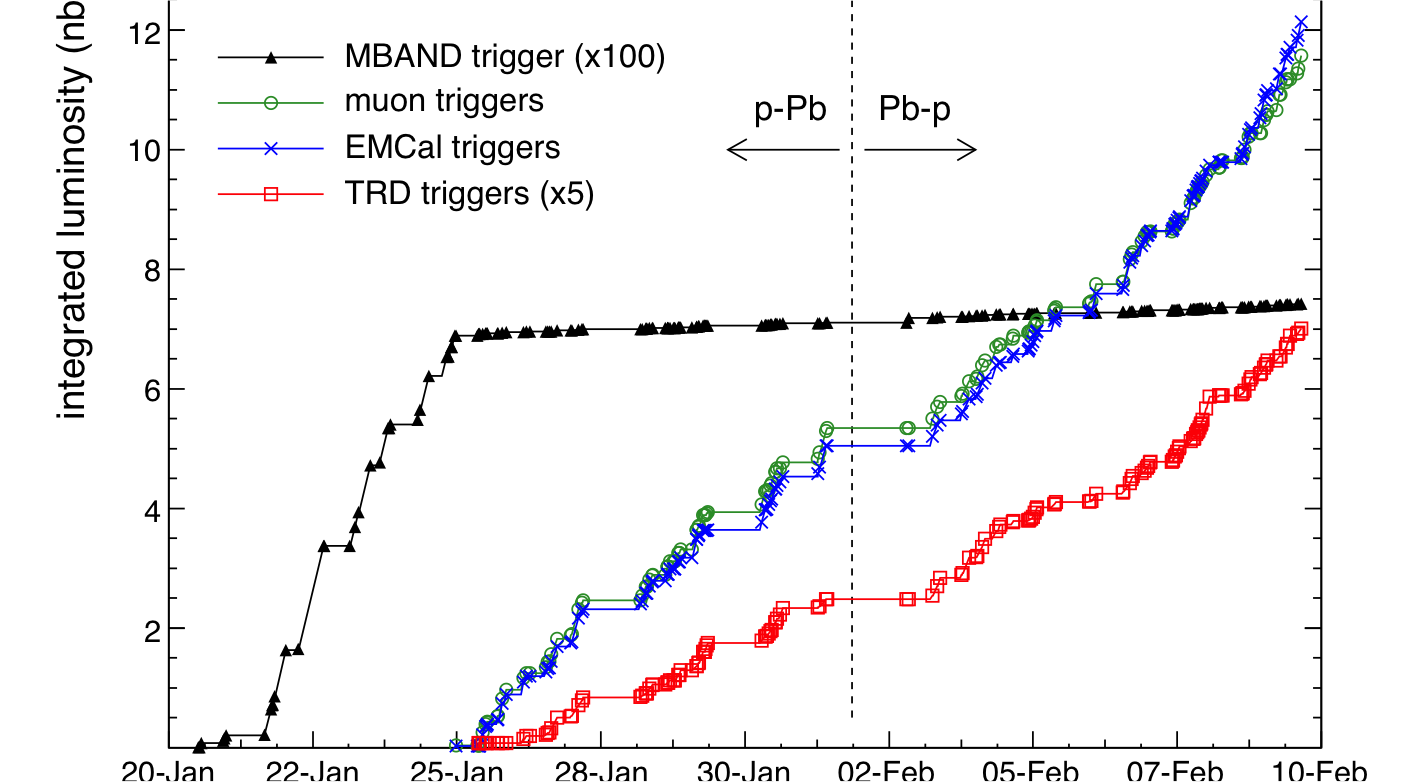
\includegraphics[width=10cm]{chap3/figure/DataSet/IntegratedLuminosity_pPb.png}
  \caption{Integrated luminosity in p-Pb collisions at $\sqrt{s_{NN}}=$5.02 TeV collected with ALICE in 2013~\cite{bib_aprrun1}.}
  \label{fig_3_luminosity}
\end{figure}


\begin{table}
  \centering
  \begin{tabular}{c|c} \hline
    Parameters             & Value                                \\ \hline
    Proton Energy          & 4 TeV                                \\
    Pb Energy              & 1.58 TeV                             \\
    Protons per bunch      & 2 $\times ~ 10^{10}$                     \\ 
    Pb ions per bunch      & 2 $\times ~10^{8}$                      \\
    Peak Luminosity        & 1 $\times ~10^{29} ~s^{-1}\rm{cm}^{-2}$       \\
    $\beta^{*}$            & 0.8                                  \\
    Transverse width       & 150 $\rm{\mu}$m                      \\
    Longitudinal emittance  & 6 cm                                 \\
    Number of Interacting Bunch & $\leq$ 338                         \\
    Collision frequency of LHC & 112.45 kHz                       \\
    Bunch spacing & 200ns                                         \\ \hline
  \end{tabular}
  \caption{Typical beam parameters for p-Pb collision in LHC Run1.}
  \label{table_3_runcondition}
\end{table}



